\documentclass{article}[IEEEtran]
\usepackage[a4paper,
            left=1in,right=1in,top=1in,bottom=0.5in,
            footskip=.25in]{geometry}
\usepackage{booktabs}
\usepackage{graphicx}
\usepackage[table,xcdraw]{xcolor}
\usepackage[utf8]{inputenc}
\usepackage{siunitx} % Provides the \SI{}{} and \si{} command for typesetting SI units
\usepackage{graphicx} % Required for the inclusion of images
\usepackage{amsmath} % Required for some math elements 
\usepackage{caption}
\usepackage{tikz}
\usepackage{import}
\usepackage{fancyhdr}
\usepackage[british]{babel}
\usepackage{algorithm}
\usepackage[noend]{algpseudocode}
\usepackage{pdfpages}
\usepackage{setspace}
\setlength\parindent{0pt} % Removes all indentation from paragraphs
\usepackage[export]{adjustbox}
\newcommand{\HRule}{\rule{\linewidth}{0.5mm}}
\usepackage{wrapfig}
\usepackage[font=scriptsize]{caption}
\usepackage{minted}
\usepackage{listings}
\definecolor{delim}{RGB}{20,105,176}
\definecolor{numb}{RGB}{106, 109, 32}
\definecolor{string}{rgb}{0.64,0.08,0.08}
\usepackage{setspace}
\usepackage{subcaption}
\usepackage{hyperref}

\lstdefinelanguage{json}{
    numbers=left,
    numberstyle=\small,
    frame=single,
    rulecolor=\color{black},
    showspaces=false,
    showtabs=false,
    breaklines=true,
    postbreak=\raisebox{0ex}[0ex][0ex]{\ensuremath{\color{gray}\hookrightarrow\space}},
    breakatwhitespace=true,
    basicstyle=\ttfamily\small,
    upquote=true,
    morestring=[b]",
    stringstyle=\color{string},
    literate=
     *{0}{{{\color{numb}0}}}{1}
      {1}{{{\color{numb}1}}}{1}
      {2}{{{\color{numb}2}}}{1}
      {3}{{{\color{numb}3}}}{1}
      {4}{{{\color{numb}4}}}{1}
      {5}{{{\color{numb}5}}}{1}
      {6}{{{\color{numb}6}}}{1}
      {7}{{{\color{numb}7}}}{1}
      {8}{{{\color{numb}8}}}{1}
      {9}{{{\color{numb}9}}}{1}
      {\{}{{{\color{delim}{\{}}}}{1}
      {\}}{{{\color{delim}{\}}}}}{1}
      {[}{{{\color{delim}{[}}}}{1}
      {]}{{{\color{delim}{]}}}}{1},
}


\lstset{language=json} 

\renewcommand{\labelenumi}{\alph{enumi}.} % Make numbering in the enumerate environment by letter rather than number (e.g. section 6)

%\usepackage{times} % Uncomment to use the Times New Roman font

            
\pagestyle{fancy}
\pagenumbering{arabic}
\fancyhf{}
\fancyfoot[C]{\thepage}
\fancyhead[L]{\nouppercase SMBUD Project - MongoDB}


\begin{document}
%===========================================================
\begin{titlepage}
\begin{center}

\captionsetup{font=footnotesize}

% Top 
\textsc{AY 2021-2022}\\[2cm]


\includegraphics[width=0.55\textwidth]{logo.png}~\\[2cm]


% Title
\HRule \\[0.4cm]
{ \LARGE 
  \textbf{SMBUD Project}\\[0.4cm]
  \emph{ELK Stack based Vaccination Campaign Analysis System}\\[0.4cm]
}
\HRule \\[1.5cm]



% Author
\begin{center}
    {\large Pablo Giaccaglia - 10626428\\[0.1cm]    Salvatore Cassata - 10560790\\[0.1cm]  Stefano Vighini - 10622788\\[0.1cm]  Zhitao He - 10763530\\[0.1cm] 
}
\end{center}

\vfill

\textsc{\large Master of Science in \\Computer Science \& Engineering}\\[0.4cm]


% Bottom
{\large \today}
 
\end{center}
\end{titlepage}

\newpage


%===========================================================
\tableofcontents
\addtocontents{toc}{\protect\thispagestyle{empty}}
\newpage
\setcounter{page}{1}

%===========================================================
%===========================================================
\section{Introduction}\label{sec:intro}

Considering the scenario in which there’s the need to build a system suitable for analysis over data about \textbf{COVID-19} vaccination statistics, we designed and build a \textbf{Kibana}\cite{b4} visualization tool relying on the \textbf{ELK stack}\cite{b2}.
The data stored allows to extract actionable insights concerning various statistical purposes, involving information such as vaccine deliveries, administered doses amounts, suppliers and age groups. The third-part data entered in the database is updated daily as it concerns vaccination campaign and so it has been also used to build insightful dashboards providing visualization at various levels of granularity.

\section{Specification \& Hypothesis}\label{sec:spec-hyp}
In order to fulfill the purpose described in the introduction, we focused on the Italian vaccination campaign by relying on the daily updated open data about delivery and administration of \textbf{COVID-19 }vaccines provided by the \textbf{Italian Ministry of Health}. Of the data available at \href{https://github.com/italia/covid19-opendata-vaccini}{this Github repository}. , only three datasets were picked to feed the system. \\\\
The idea is to provide a tool aware of data updates, reason for why we implemented a small data processing pipeline to fetch, slightly change and standardize the data uploaded to the aforementioned repository. More details about this process will be provided in the next sections.

\section{Data schema}\label{sec:data-schema}

In the following subsections the three used datasets are now showed from the structural point of view and briefly described.

\subsection{"somministrazioni-vaccini-latest" dataset}

Italian vaccination campaign data of daily administered vaccines divided by region and age group of the vaccinated subjects. The shape of the data is the same as in the one of the Github repository, with the exception of translated fields from Italian to English and the addition of the \textbf{"region\_coordinates"} field. More details about these changes are shown in section \ref{sec:creation}.

\begin{table}[H]
\centering
\begin{tabular}{@{}lll@{}}
\toprule
\textbf{Field}         & \textbf{Data type} & \textbf{Description}                                                                                               \\ \midrule
administration\_date   & Date               & Administration date of the vaccines                                                                                \\ 
\rule{0pt}{3ex}%  EXTRA vertical height  
supplier               & Keyword            & Complete name of the supplier of the vaccine                                                                       \\
\rule{0pt}{3ex}%  EXTRA vertical height 
area                   & Text               & Acronyms of the region of delivery                                                                                 \\
\rule{0pt}{3ex}%  EXTRA vertical height 
age\_group             & Keyword            & Age group of the people administered with the vaccine                                                              \\
\rule{0pt}{3ex}%  EXTRA vertical height 
male\_count            & Integer            & Number of vaccinations administered to males                                                                       \\
\rule{0pt}{3ex}%  EXTRA vertical height 
female\_count          & Integer            & Number of vaccinations administered to females                                                                     \\
\rule{0pt}{3ex}%  EXTRA vertical height 
first\_doses           & Integer            & Number of people administered with first dose                                                                      \\
\rule{0pt}{3ex}%  EXTRA vertical height 
second\_doses          & Integer            & Number of people administered with second dose                                                                     \\
\rule{0pt}{5ex}%  EXTRA vertical height 
post\_infection\_doses & Integer            & \begin{tabular}[c]{@{}l@{}}Number of people administered with a dose after \\ they have been infected in the previous 3-6 months\end{tabular} \\
\rule{0pt}{5ex}%  EXTRA vertical height 
booster\_doses         & Integer            & \begin{tabular}[c]{@{}l@{}}Number of people administered with an additional\\ dose/recall\end{tabular}             \\
\rule{0pt}{5ex}%  EXTRA vertical height 
NUTS1\_code            & Text               & \begin{tabular}[c]{@{}l@{}}NUTS (Nomenclature of Territorial Units for Statistics) \\ code 1 of Italy\end{tabular} \\
\rule{0pt}{5ex}%  EXTRA vertical height 
NUTS2\_code            & Text               & \begin{tabular}[c]{@{}l@{}}NUTS (Nomenclature of Territorial Units for Statistics) \\ code 2 of Italy\end{tabular} \\
\rule{0pt}{3ex}%  EXTRA vertical height 
region\_ISTAT\_code    & Integer            & ISTAT region code                                                                                                  \\
\rule{0pt}{3ex}%  EXTRA vertical height 
region\_name           & Keyword            & Name of the region                                                                                                 \\
\rule{0pt}{3ex}%  EXTRA vertical height 
region\_coordinates    & Geo point          & Latitude-longitude pair of region coordinates                                                                      \\ \bottomrule
\end{tabular}
\end{table}


\subsection{"anagrafica-vaccini-summary-latest" dataset}


Italian vaccination campaign data of overall administered vaccines, including female and male count. The shape of the data is the same as in the one of the Github repository, with the exception of translated fields from Italian to English. More details about these changes are shown in section \ref{sec:creation}.

\begin{table}[H]
\centering
\begin{tabular}{lll}
\hline
\textbf{Field}         & \textbf{Data type} & \textbf{Description}                                                                                                                                 \\ \hline
age\_group             & Keyword            & Age group of vaccinated people                                                                                                                       \\
\rule{0pt}{3ex}%  EXTRA vertical height 
total\_administered    & Integer            & Overall amount of administered vaccine doses                                                                                                         \\
\rule{0pt}{3ex}%  EXTRA vertical height 
male\_count            & Integer            & Overall number of vaccinations administered to males                                                                                                 \\
\rule{0pt}{3ex}%  EXTRA vertical height 
female\_count          & Integer            & Overall number of vaccinations administered to females                                                                                               \\
\rule{0pt}{3ex}%  EXTRA vertical height 
first\_doses           & Integer            & Overall number people administered with first dose                                                                                                   \\
\rule{0pt}{3ex}%  EXTRA vertical height 
second\_doses          & Integer            & Overall number people administered with second dose                                                                                                  \\
\rule{0pt}{5ex}%  EXTRA vertical height 
post\_infection\_doses & Integer            & \begin{tabular}[c]{@{}l@{}}Overall number of people administered with a dose after\\ they have been infected in the previous 3-6 months\end{tabular} \\
\rule{0pt}{5ex}%  EXTRA vertical height 
booster\_doses         & Integer            & \begin{tabular}[c]{@{}l@{}}Overall number of people administered with an additional\\ dose/recall\end{tabular}                                       \\
\rule{0pt}{3ex}%  EXTRA vertical height 
last\_update           & Date               & Latest update date             
 \\ \bottomrule
 
\end{tabular}
\end{table}

\subsection{"consegne-vaccini-latest" dataset}

Italian vaccination campaign data of daily delivered vaccines divided by region and supplier. The shape of the data is the same as in the one of the Github repository, with the exception of translated fields from Italian to English and the addition of the \textbf{"region\_coordinates"} field. More details about these changes are shown in section \ref{sec:creation}.

\begin{table}[H]
\centering
\begin{tabular}{@{}lll@{}}
\toprule
\textbf{Field}      & \textbf{Data type} & \textbf{Description}                                                                                               \\ \midrule
area                & Text               & Acronyms of the region of delivery                                                                                 \\
\rule{0pt}{3ex}%  EXTRA vertical height 
supplier            & Keyword            & Complete name of the supplier of the vaccine                                                                       \\
\rule{0pt}{3ex}%  EXTRA vertical height 
doses\_amount       & Integer            & Number of  delivered doses                                                                                         \\
\rule{0pt}{3ex}%  EXTRA vertical height 
delivery\_date      & Date               & Date of the delivery                                                                                               \\
\rule{0pt}{5ex}%  EXTRA vertical height 
NUTS1\_code         & Text               & \begin{tabular}[c]{@{}l@{}}NUTS (Nomenclature of Territorial Units for Statistics) \\ code 1 of Italy\end{tabular} \\
\rule{0pt}{5ex}%  EXTRA vertical height 
NUTS2\_code         & Text               & \begin{tabular}[c]{@{}l@{}}NUTS (Nomenclature of Territorial Units for Statistics) \\ code 2 of Italy\end{tabular} \\
\rule{0pt}{5ex}%  EXTRA vertical height 
region\_ISTAT\_code & Integer            & ISTAT region code                                                                                                  \\
\rule{0pt}{3ex}%  EXTRA vertical height 
region\_name        & Keyword            & Name of the region                                                                                                 \\
\rule{0pt}{3ex}%  EXTRA vertical height 
region\_coordinates & Geo point          & Latitude-longitude pair of region coordinates                                                                      \\ \bottomrule
\end{tabular}
\end{table}

\newpage

\section{Database Creation}\label{sec:creation}

As stated in the introduction section, we decided to build a Python\cite{b5} data pipeline to provide a daily database update, while ensuring to be consistent with the modifications we applied to the original datasets. Obviously a manual approach isn't feasible for this purpose, so different steps taken into account by the daily routines are now briefly explained, referencing to a real use case scenario.

\begin{figure}[H]
\begin{center}
    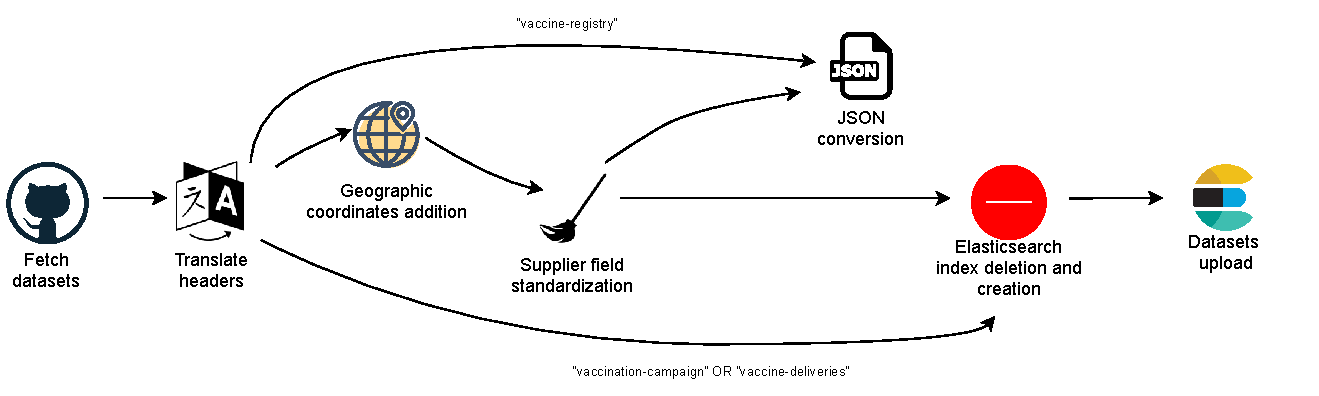
\includegraphics[width=0.95\textwidth]{pipeline.pdf}
    \caption{Pipeline steps}
\end{center}
\end{figure}

\begin{itemize}
    \item \textbf{Datasets fetch from Github repository}: \textbf{CSV files} are updated every day at around \textbf{5:15 AM}, then some sort of watcher-notifier tool (not integrated at the moment), such as \textbf{GitHub File Watcher}\cite{b6}, could trigger the daily routines functions (implemented), whose first step is the files fetch for processing.
    
    \item \textbf{CSV Header translation}: the original CSV files' headers are in Italian, so we decided to translate them in English to widen the audience of users. This modification doesn't affect the content of the datasets and it is easily adaptable to header names changes, since the translation is performed daily through a lookup table (\textbf{Python Enum subclass}) which can be easily changed through add-ons, modifications and deletions.
    File names were also translated, and the resulting names are: "vaccination-campaign" for \textbf{"somministrazioni-vaccini-latest"}, \textbf{"vaccine-registry"} for \textbf{"anagrafica-vaccini-summary-latest"} and "vaccine-deliveries" for  \textbf{”consegne-vaccini-latest”}. Note that these translations correspond to the \textbf{Elasticsearch}\cite{b3} Indexes names and from now these document and their fields will be named after their English translation.
    
    \item \textbf{Adding region coordinates}: This addition is performed only on \textbf{"vaccine-deliveries"} and \\ \textbf{"vaccination-campaign"} datasets, since these contain a \textbf{"region\_name"} field, through which is possible to associate the corresponding region coordinates as a pair. The coordinates are retrieved from a previously created file containing mappings of Italian regions to their corresponding coordinates, retrieved through the \textbf{GMaps Geocoding API}\cite{b1}. This information doesn't alter the original data and is used to provide \textbf{Kibana} Geo data visualizations of the vaccination campaign. Note that this operation is performed by a Python function that lets choosing the way in which the data is added: through a single CSV column named \textbf{"region\_coordinates"} or through 2 CSV columns named \textbf{"region\_longitude"} and \textbf{"region\_latitude"}, containing the corresponding float values.
    This addition is compatible with the daily updates, since we assume that it is unlikely a change of the \textbf{"region\_name"} filed values. But if there will be such case, for example concerning lower/upper case characters, it is almost immediate to face it by changing the lookup table region names, or by writing appropriate functions to face multiple scenarios.
    
    \item \textbf{Supplier filed "standardization"}: This is the only significant modification we applied to two of the original datasets: \textbf{"vaccination-campaign"} and \textbf{"vaccine-deliveries"}. The alteration involves \textbf{"supplier"} field of both datasets, whose values are the names of vaccine's suppliers, e.g: \\ \textbf{Pfizer/BioNTech, Moderna}. In detail among the possible values of this textual field there are \\ \textbf{"Pfizer/BioNTech"} and \textbf{"Pfizer Pediatrico"}, that is "Pediatric Pfizer". Since we don't consider this distinction meaningful for the insight we want to provide the user through this system, we decided to standardize both fields under the name of the former. Note that also in this case same reasoning done for the previous step concerning daily updates and format changes can be applied.
    
    \item \textbf{Datasets upload to Elasticsearch}: After the data manipulation phase, some additional steps are taken to successfully upload the data. Firstly the three indexes, if previously created, are deleted from Elasticsearch, then recreated to upload the newer data from the final CSVs. This step, which could sound not optimal, is taken because we noticed eventual updates of older data (e.g number of doses amount was partial). Even though more sophisticated solutions involving detection changes methods and upload of only new/changed entries could be adopted, we didn't do that to focus on other aspects of the project.
    
    \item \textbf{Additional notes}: Through the provided Python routines in the last step of the process, final CSVs are converted to Json format for eventual further usages. The datasets are uploaded online through \textbf{Elasticsearch DSL Python library}, manual mapping is performed in this phase for 2 reasons: aim to have uploaded data ready for interaction without further tweaks and to have full control on data types, to avoid eventual unwanted automatic mappings and to specify Keyword fields, to perform aggregation both in Elasticsearch queries and Kibana dashboards on textual fields.
    
\end{itemize}

\newpage

\section{Kibana dashboard panels}\label{sec:dashboard}

In the following chapter we are describing the Kibana dashboards we implemented. We used different indexes and we also tried to cover different ways of \textbf{representation} (bar charts, maps, pie charts) and different \textbf{functions} (cumulative sums, total sums, daily data). Most of the dashboards are \textbf{interactive}: this means you can select an interval with the left click of the mouse and the graph will zoom into it; or for other types you can select/deselect some data (for example, in the map).

Note that even though in Italy the first vaccine against \textbf{COVID-19} was administered on \textbf{27/12/2020}, the following charts, when the \textbf{x-axis} is divided into week intervals, the starting week is on \textbf{21/12/2020.}

\subsection{Gender distribution of weekly vaccine doses administered}\label{ssec:dash1}

This bar chart shows the amount of vaccine doses administered each week, from the one starting on \textbf{21/12/2020}.
The shown amounts are based uniquely on the overall doses, the only distinction made is in the gender of vaccinated people. Note that if daily database updates occur, the current week's bar may refer partial amounts. Thanks to Kibana tools, week range can be customized, impacting the \textbf{x-axis}, and fields can be hidded to shift the focus on a portion of them. This chart relies on the \textbf{"vaccination-campaign"} index and its data can be obtained through the query shown at subsection \ref{ssec:q3}

\begin{figure}[H]
\begin{center}
    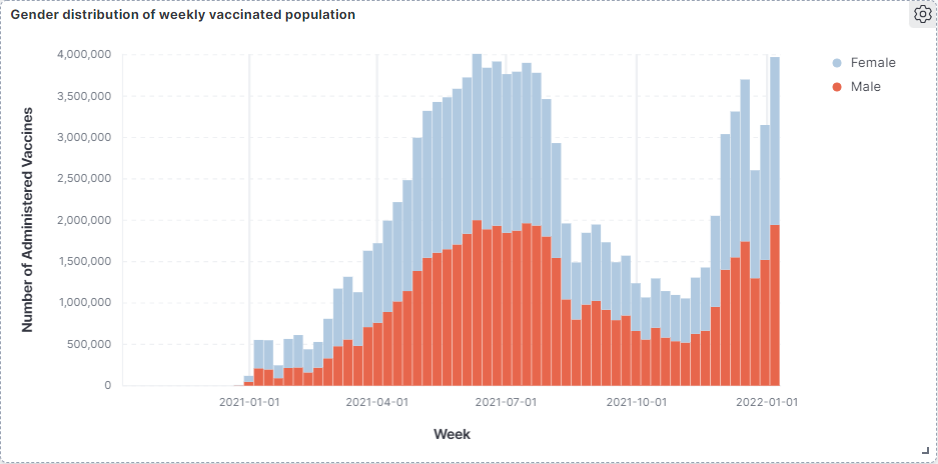
\includegraphics[width=0.7\textwidth, frame]{Gender distribution of weekly vaccine doses administered.png}
    \caption{Gender distribution of weekly vaccine doses administered}
\end{center}
\end{figure}



\subsection{Number of not vaccinated people}\label{ssec:dash2}

This bar chart shows the decrease of overall amount of not vaccinated people each week, from the one starting on \textbf{21/12/2020}.
The shown amounts are based uniquely on the cumulative sum of first doses. Note that, since it is not possible to have some sort of tool able to provide the current population given the filters applicable on the data,
the values shown are computed by subtracting the cumulative sum from the overall Italian population value (\textbf{60,327,146}), which is hardcoded. 
Finally note that the number of not vaccinated people includes not vaccinable people.
This chart relies on the \textbf{"vaccination-campaign"} index and its data can be obtained through the query shown at subsection \ref{ssec:q7}

\begin{figure}[H]
\begin{center}
    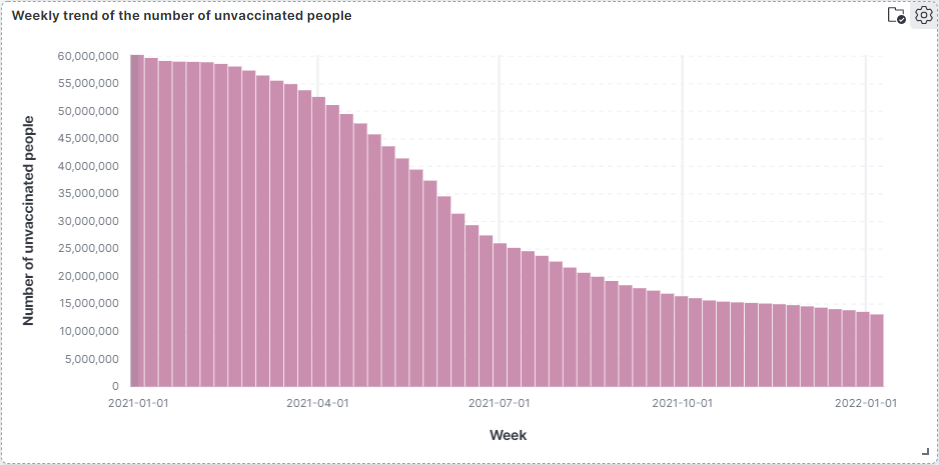
\includegraphics[width=0.7\textwidth, frame]{Number of not vaccinated people.png}
    \caption{Number of not vaccinated people}
\end{center}
\end{figure}


\subsection{Weekly trend of the number of vaccinations}\label{ssec:dash3}

This line chart shows the amount of vaccine doses administered each week, from the one starting on \textbf{21/12/2020}. The shown amount doesn't consider distinction between males and females, but uniquely the distinction between first, second and booster dose. Thanks to Kibana tools, week range can be customized, impacting the \textbf{x-axis}, and fields can be hided to shift the focus on a portion of them. This chart relies on the \textbf{"vaccination-campaign"} index and its data can be obtained through the query shown at subsection \ref{ssec:q1}

\begin{figure}[H]
\begin{center}
    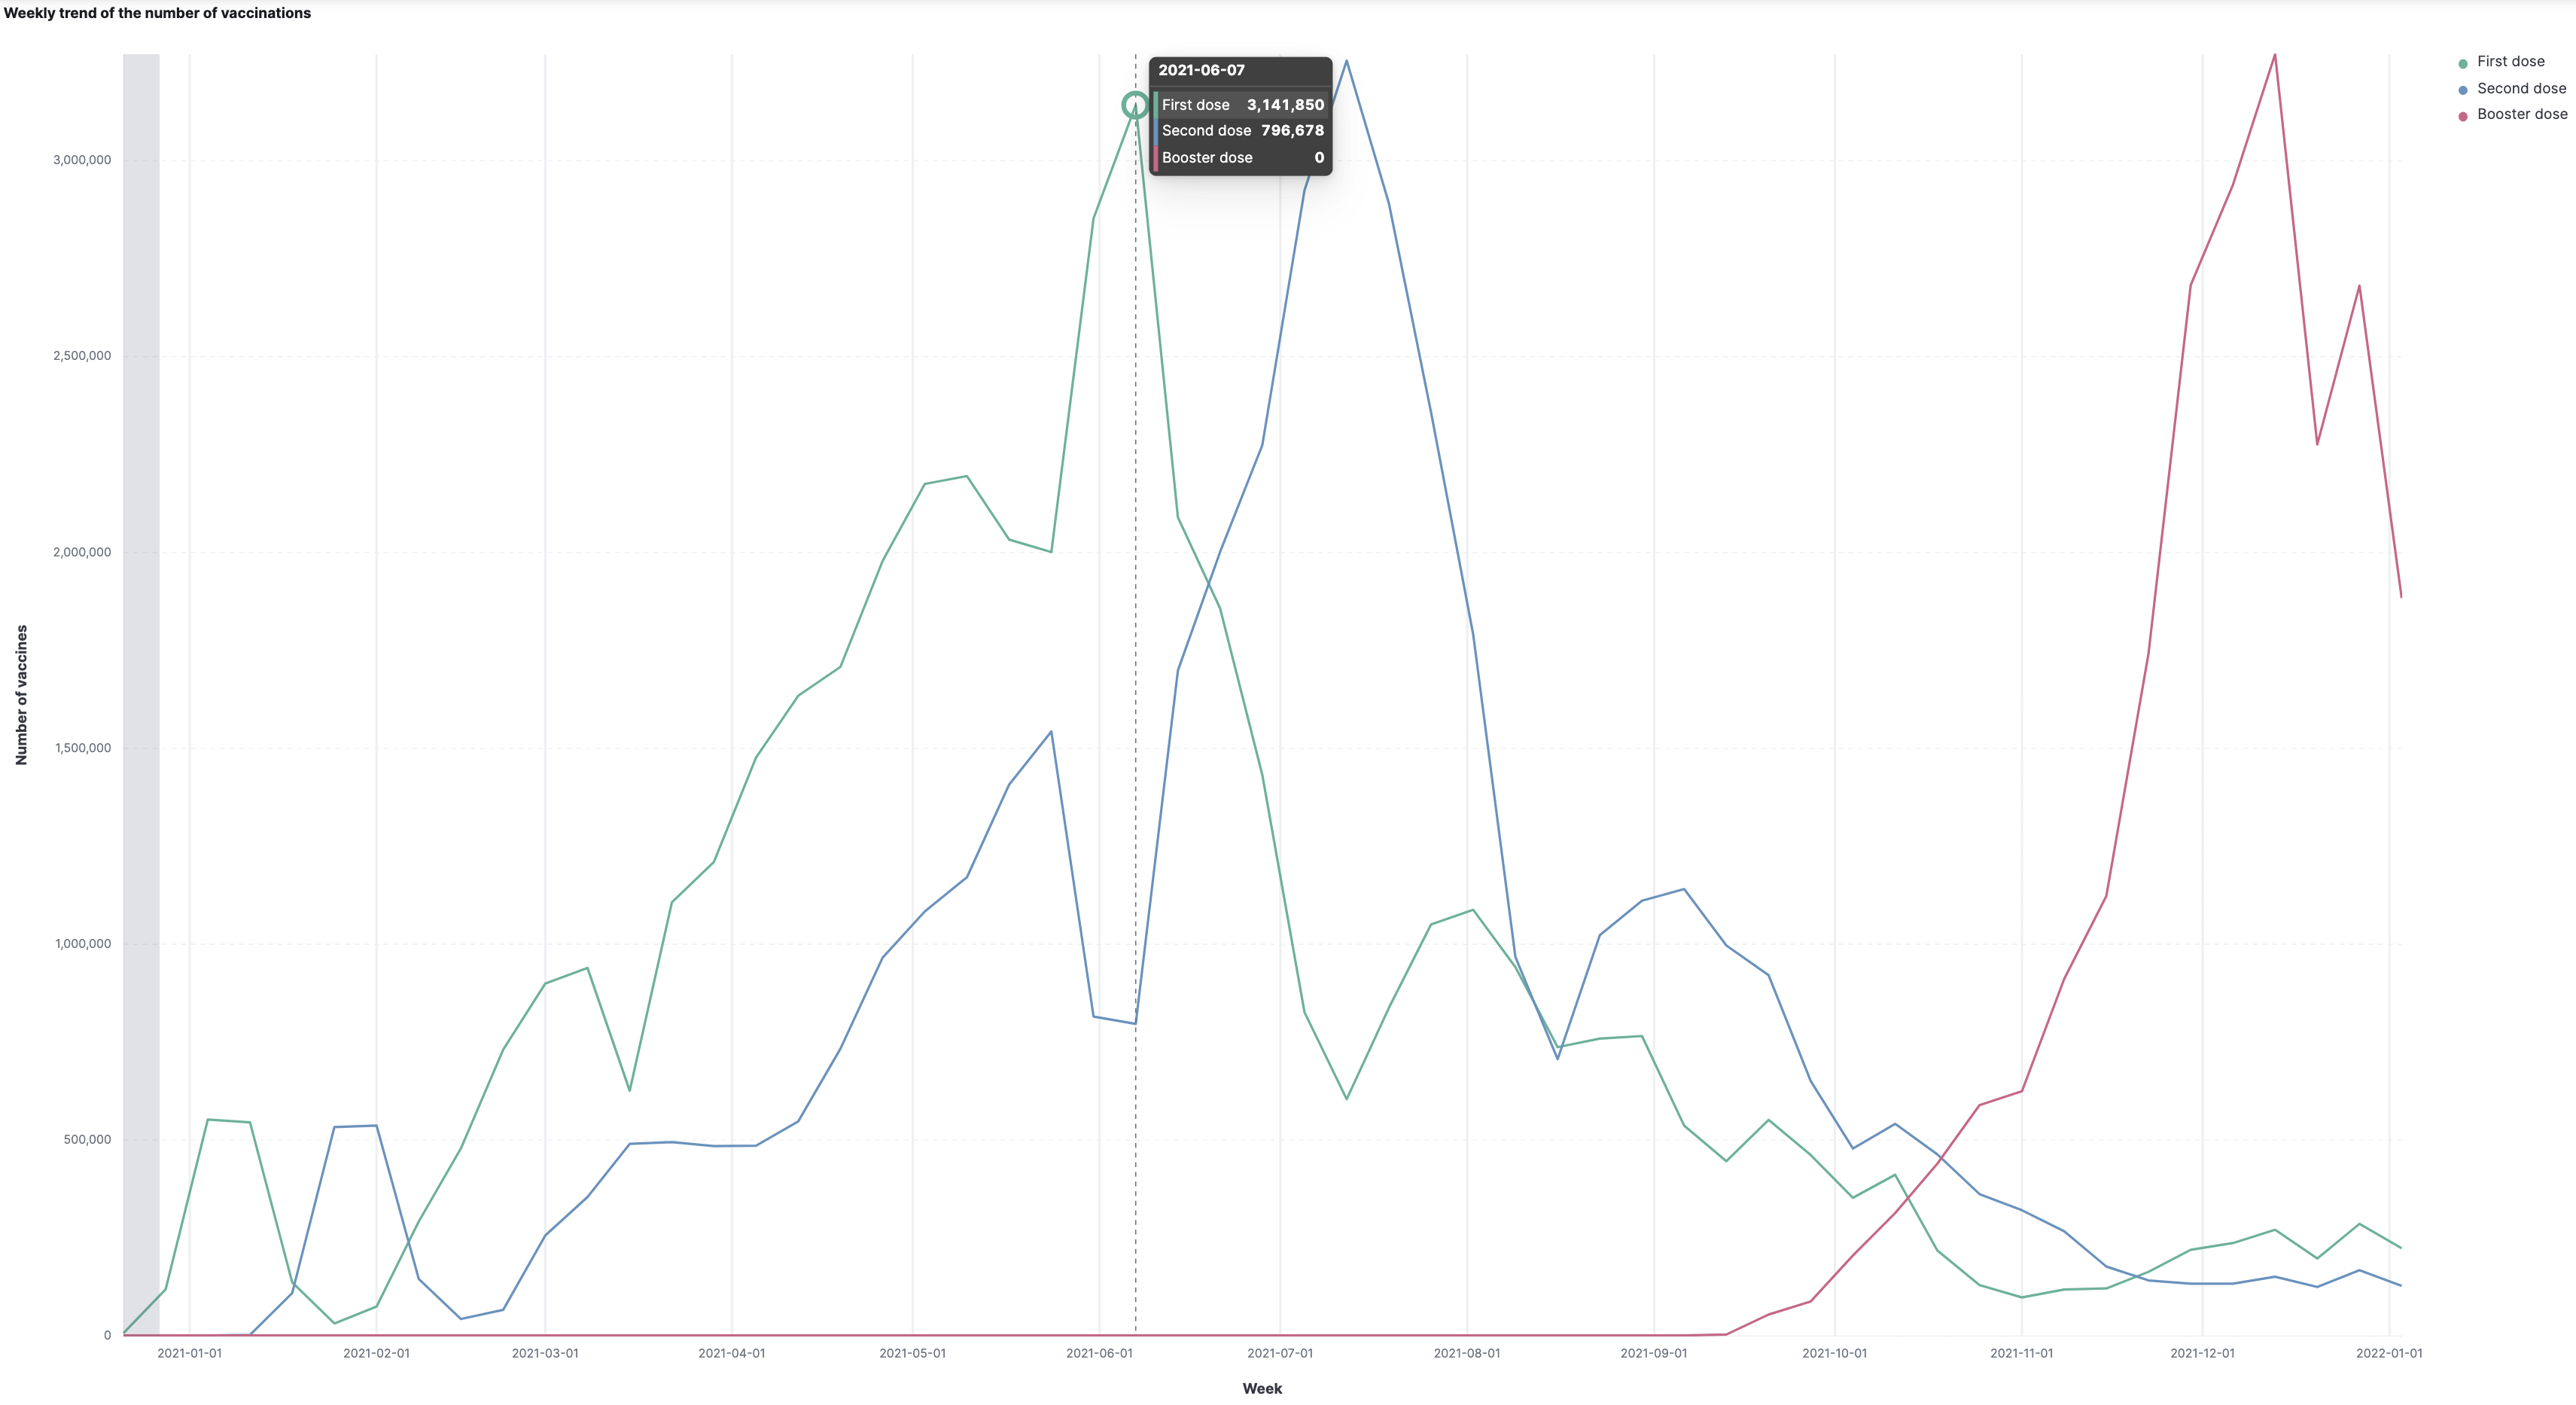
\includegraphics[width=0.95\textwidth, frame]{Weekly trend of the number of vaccinations.png}
    \caption{Weekly trend of the number of vaccinations}
\end{center}
\end{figure}

\subsection{Total number of doses delivered}\label{ssec:dash4}

This area chart shows the increase of overall amount of vaccines delivered each week, from the one starting on \textbf{21/12/2020}.
The shown amount doesn't consider distinction between suppliers.  Thanks to Kibana tools, week range can be customized, impacting the \textbf{x-axis}. This chart relies on the \textbf{"vaccine-deliveries"} index and its data can be obtained through the query shown at subsection \ref{ssec:q11}.

\begin{figure}[H]
\begin{center}
    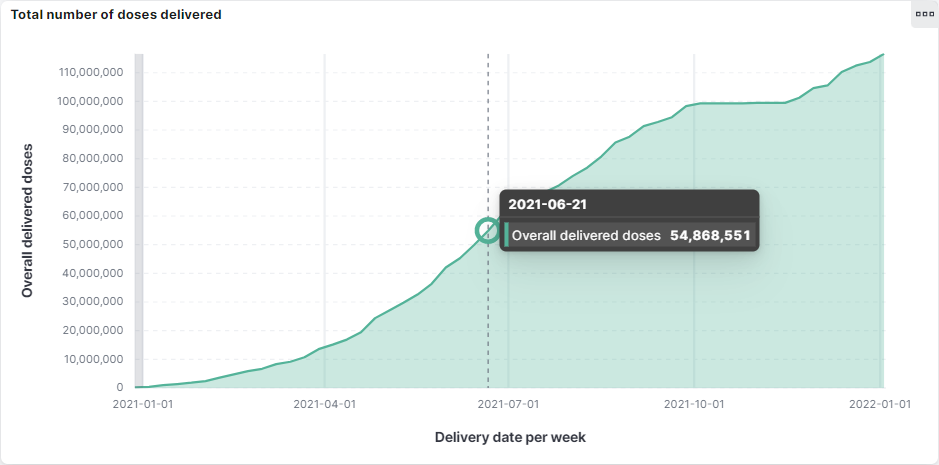
\includegraphics[width=0.95\textwidth, frame]{Total number of doses delivered.png}
    \caption{Total number of doses delivered}
\end{center}
\end{figure}

\newpage

\subsection{Distribution of suppliers of all administered vaccines}\label{ssec:dash5}

This pie chart shows the distribution of doses administered from the supplier point of view. The shown amount doesn't consider distinction between males and females, nor the distinction between first, second and booster dose. The shown amounts are based uniquely on the cumulative sum of first, second and booster doses. 
Thanks to Kibana tools, date range can be customized, impacting the chart aspect and allowing to focus on the distribution trend of a certain period of time. This chart relies on the \textbf{"vaccination-campaign"} index and its data is the one obtained through the query shown at subsection \ref{ssec:q4}. 

\begin{figure}[H]
\begin{center}
    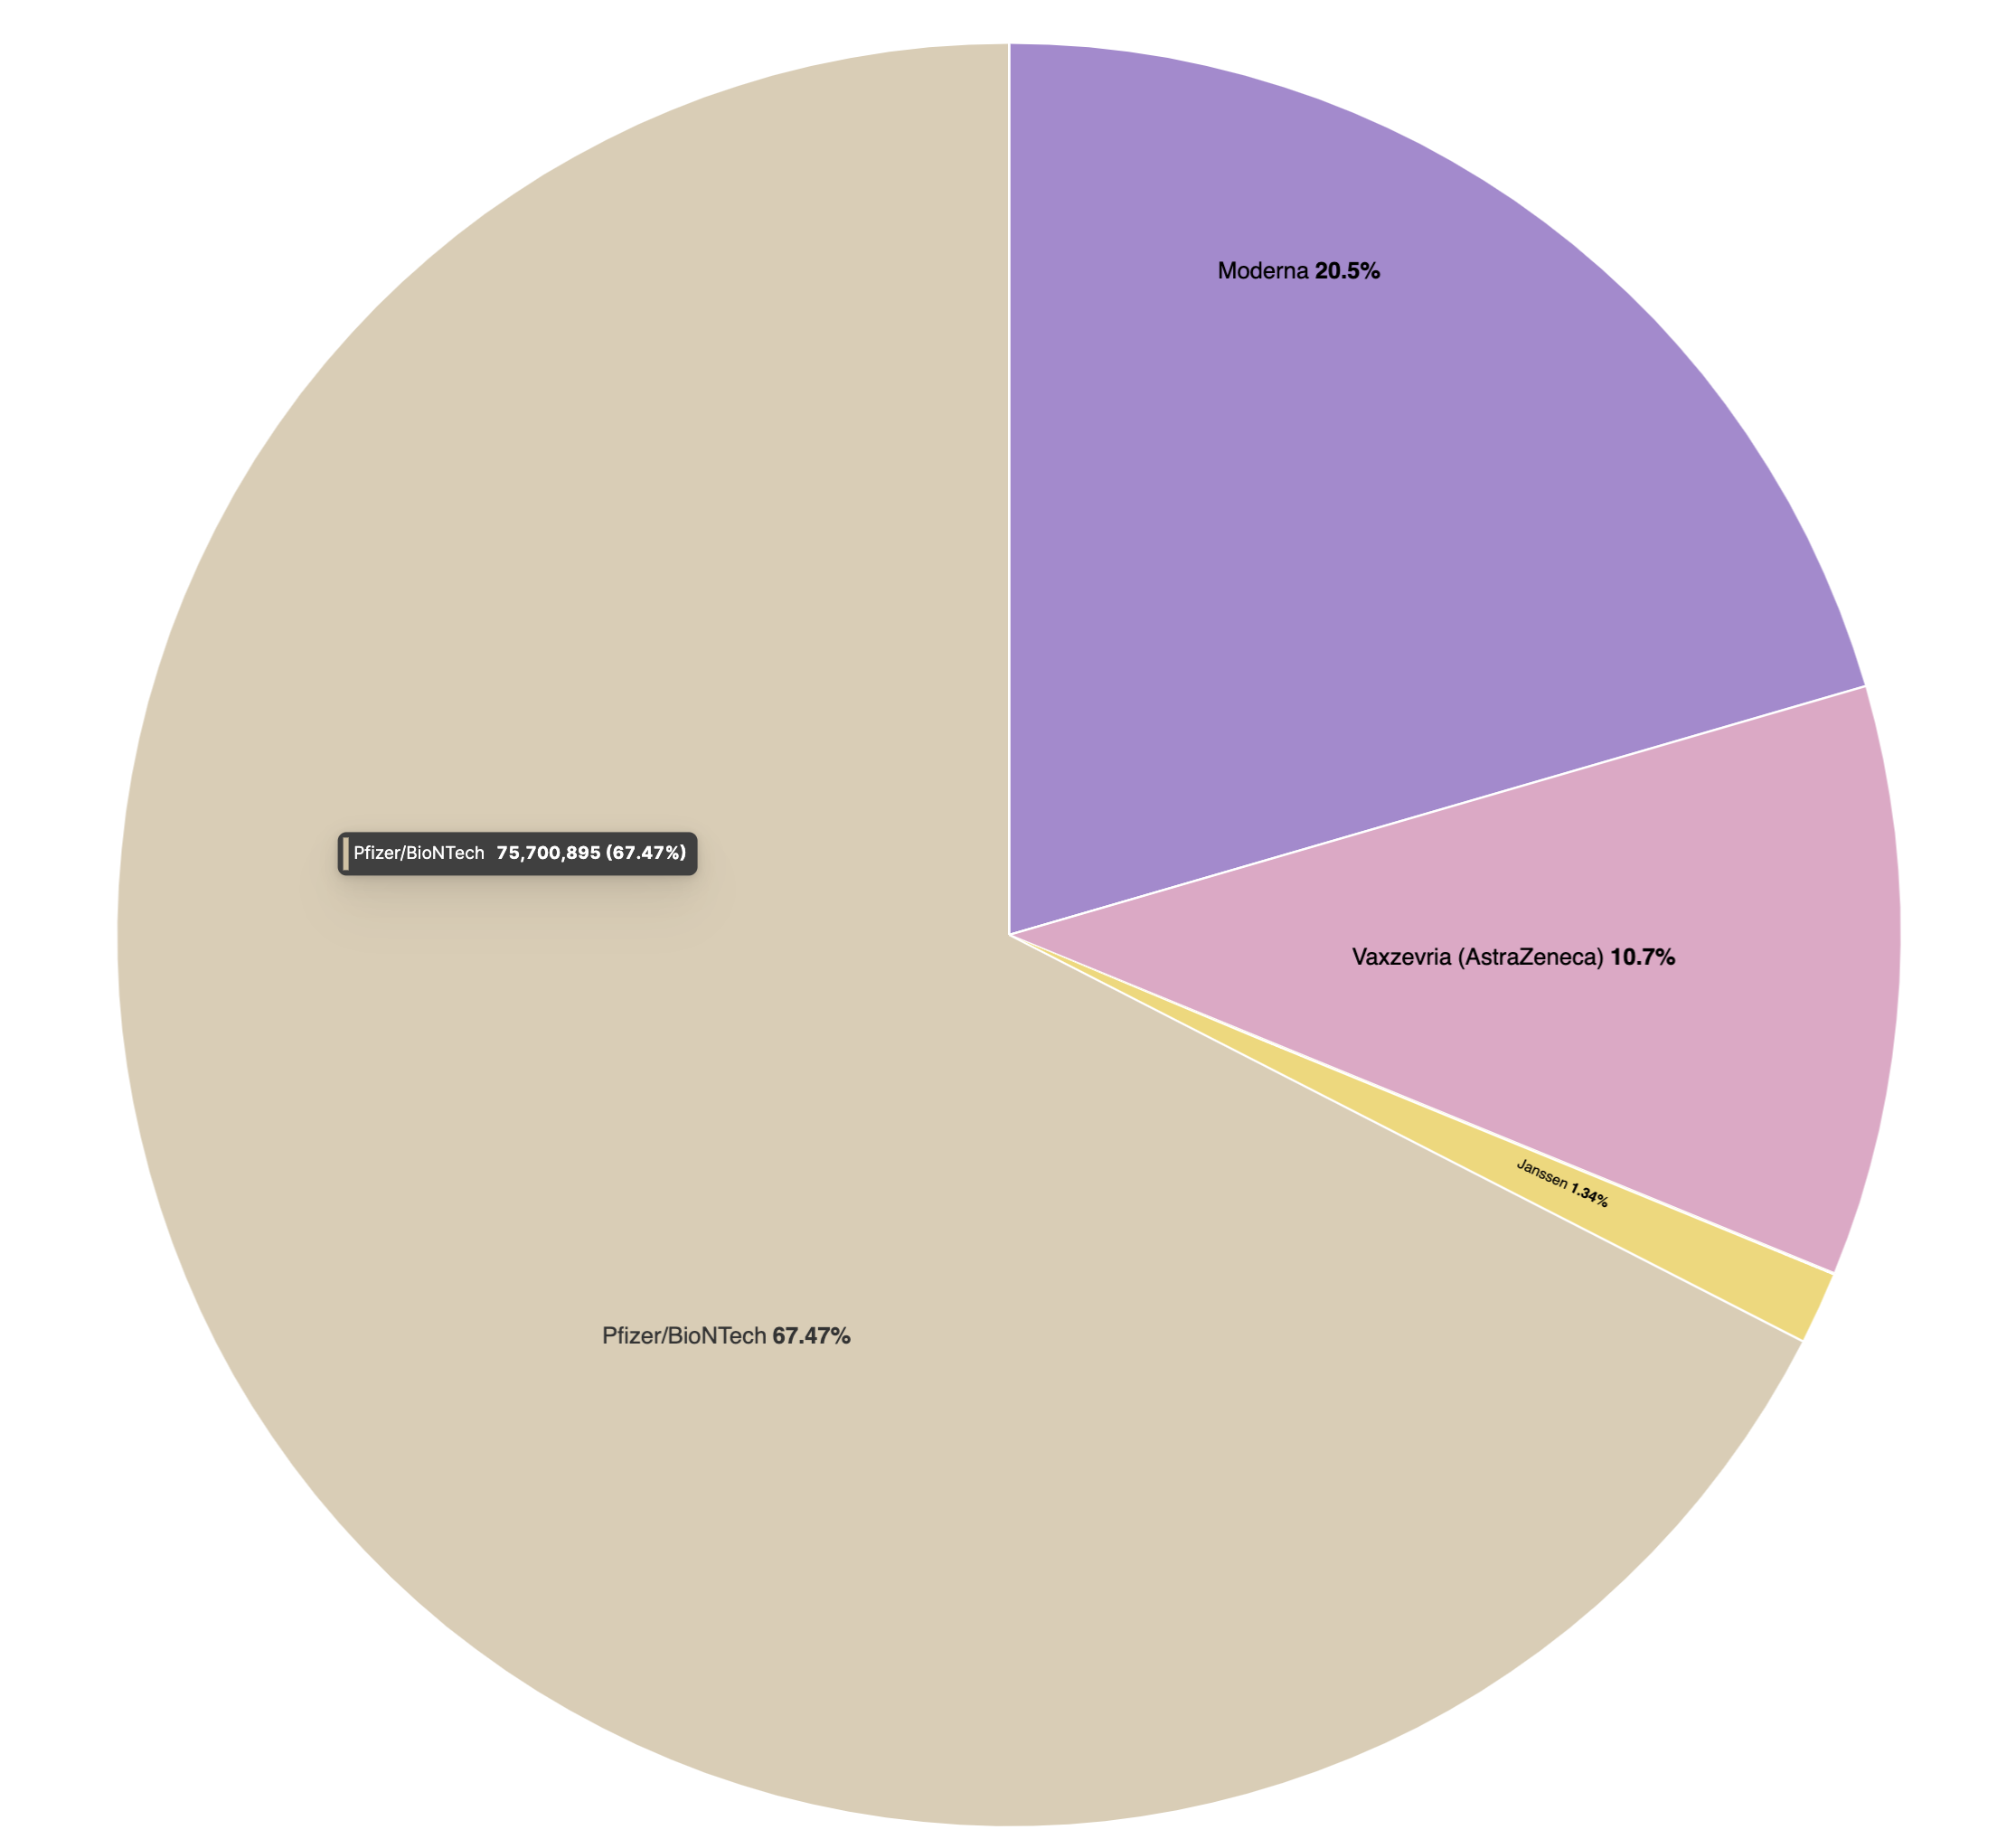
\includegraphics[width=0.5\textwidth, frame]{Distribution of suppliers of all administered vaccines.png}
    \caption{Distribution of suppliers of all administered vaccines}
\end{center}
\end{figure}

\subsection{Vaccination status of all age groups}\label{ssec:dash6}

This bar chart shows the vaccination status of all age groups, considering percentages relative to the people who got at least one vaccine, to compute the ones relative to both people waiting the second dose, the booster dose and the ones fully vaccinated. Not vaccinated people are not considered. \textbf{"waiting for taking the second dose"} percentages are computed considering the difference between the sum of first doses and second doses, by age range. \textbf{"waiting for taking the booster dose"} percentages are computed considering the difference between the sum of second doses and booster doses, by age range. Finally the \textbf{"fully vaccinated"} percentage is simply the sum of booster doses administered, by age range. 
Thanks to Kibana tools, week range can be customized, impacting the \textbf{x-axis}, and fields can be hidded to shift the focus on a portion of them.
This chart relies on the "vaccination-campaign" index and its data can be obtained through the query shown at subsection \ref{ssec:q6}

\begin{figure}[H]
\begin{center}
    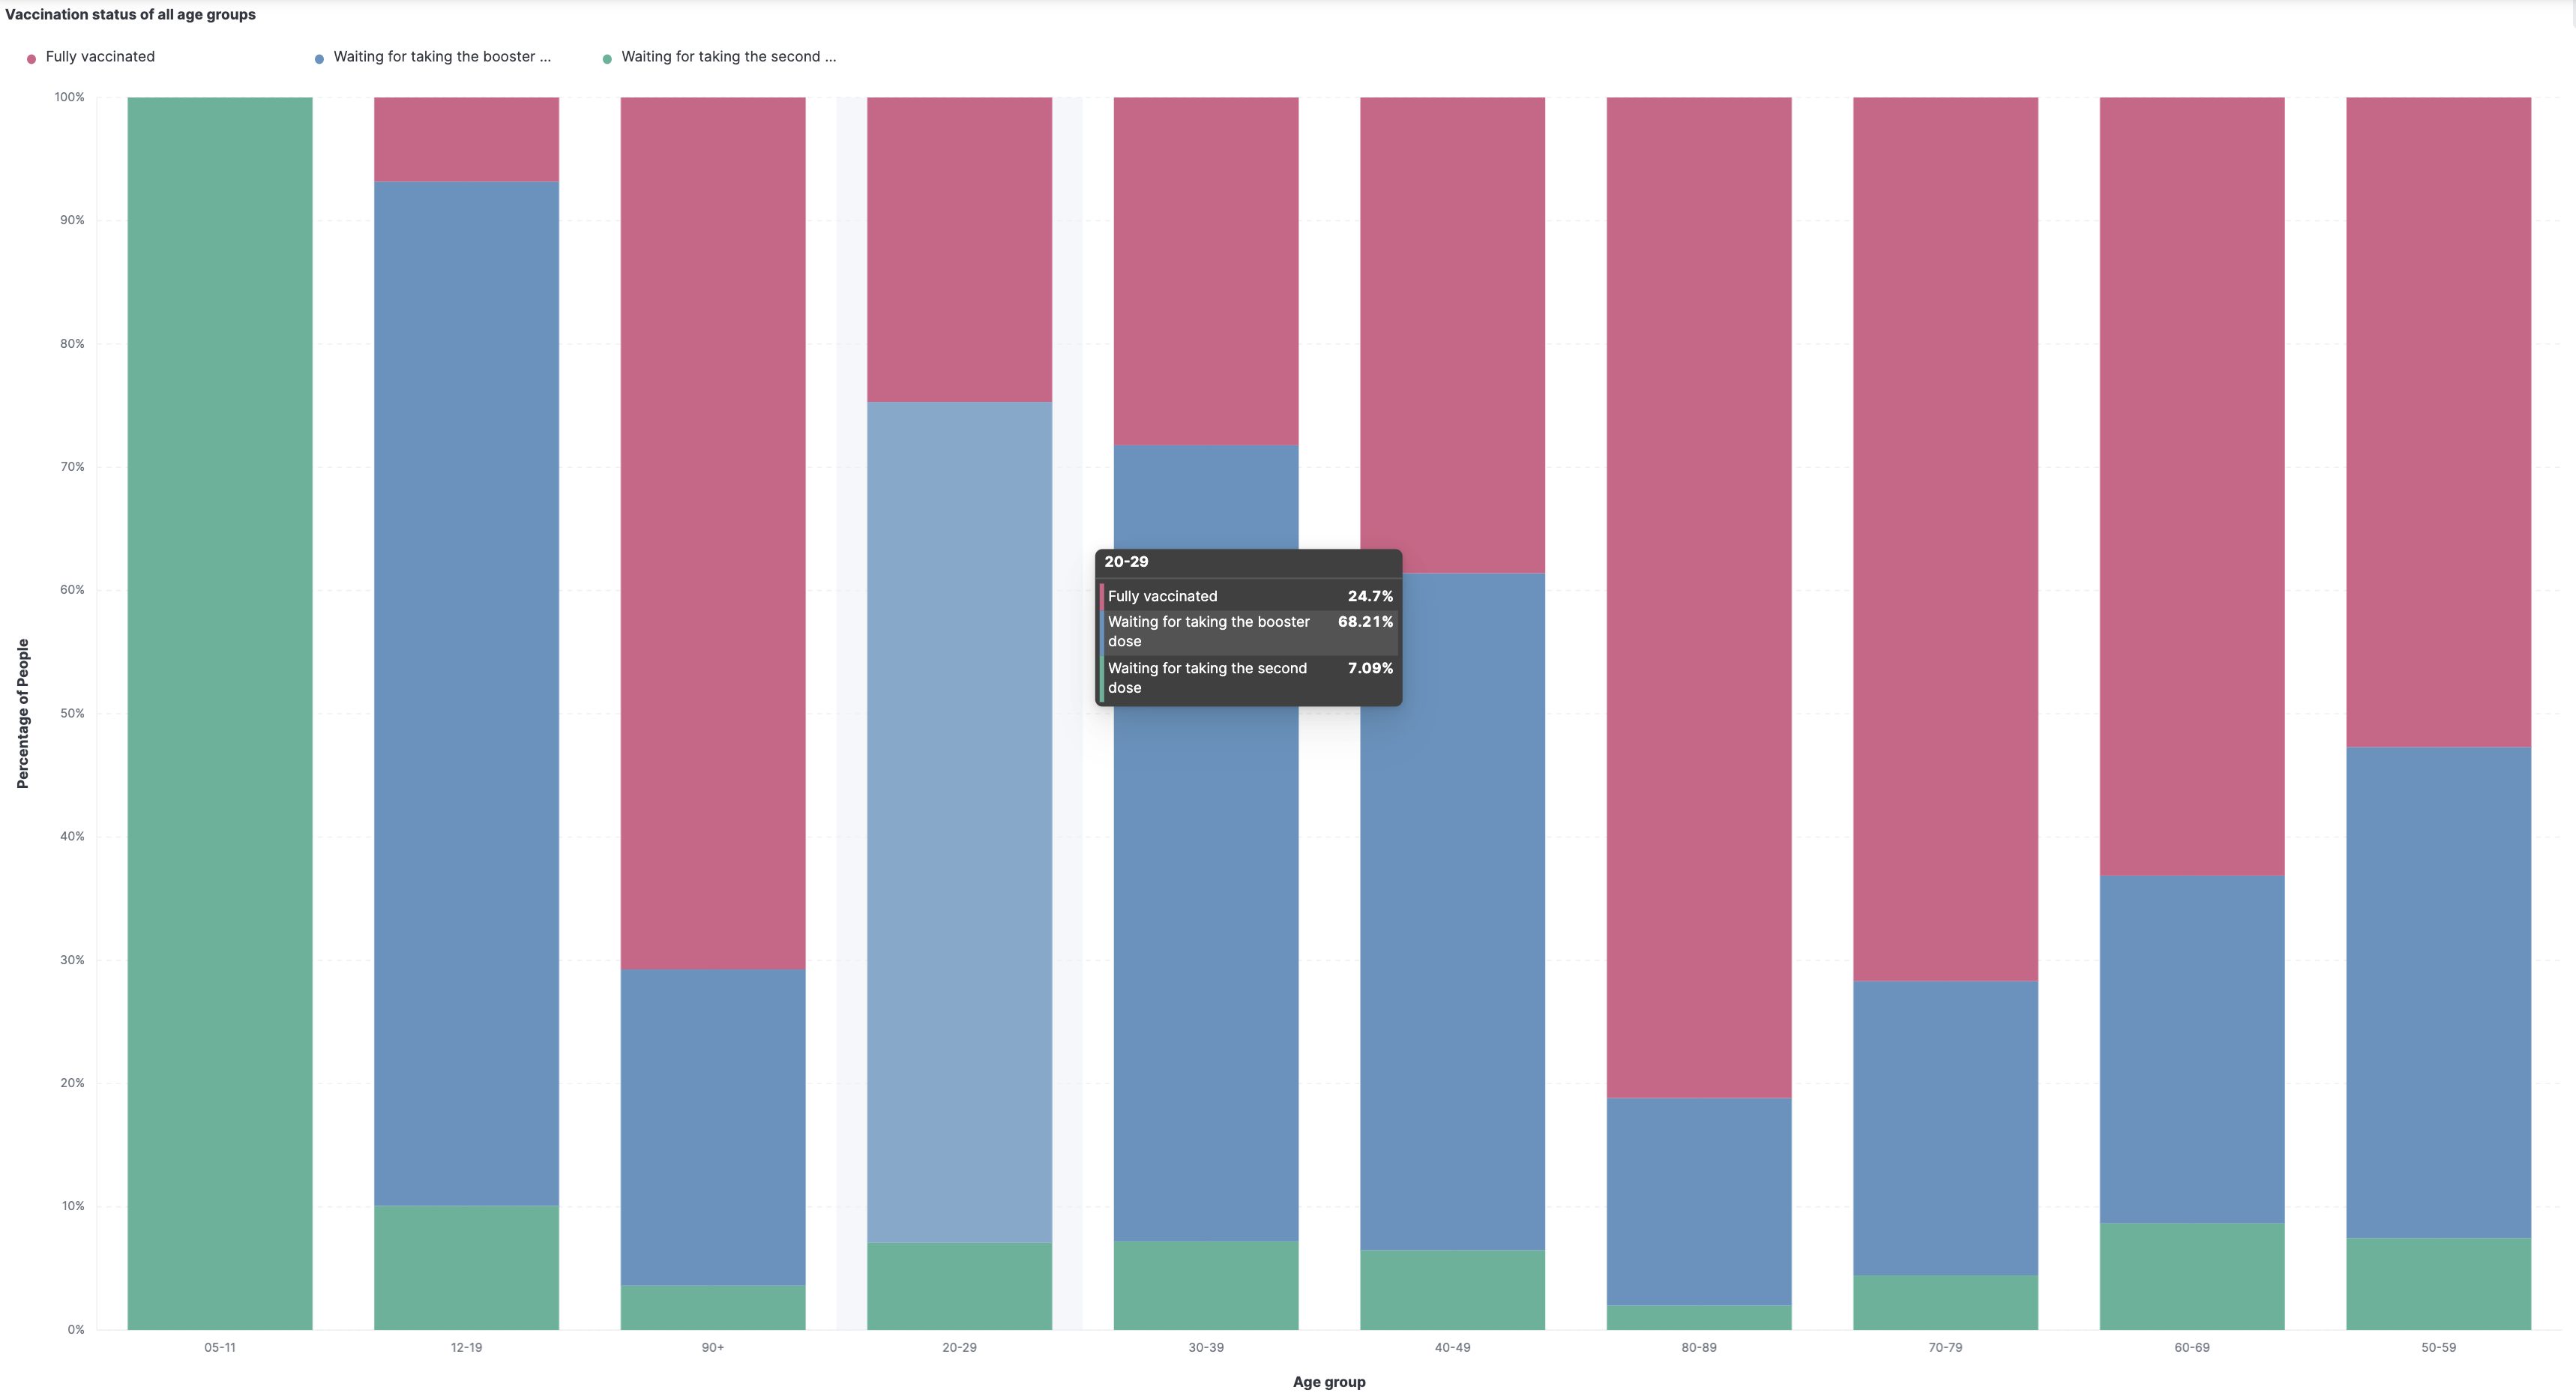
\includegraphics[width=0.7\textwidth, frame]{Vaccination status of all age groups.png}
    \caption{Vaccination status of all age groups}
\end{center}
\end{figure}

\subsection{Doses map}\label{ssec:dash7}

This map shows the total number of doses delivered from the start of the pandemic up to now. As you can see, bigger amounts of doses delivered correspond to bigger circles with a red color, while smaller amounts to smaller circles with green color. On the left, you can see multiple layers for this map have been created, just to show you it's possible to show more data at once and to hide some layers. However, this is not useful in our case as the region coordinates make this layers overlap and not effectively readable. The data of the map can be retrieved by query \ref{ssec:q15}.

\begin{figure}[H]
\begin{center}
    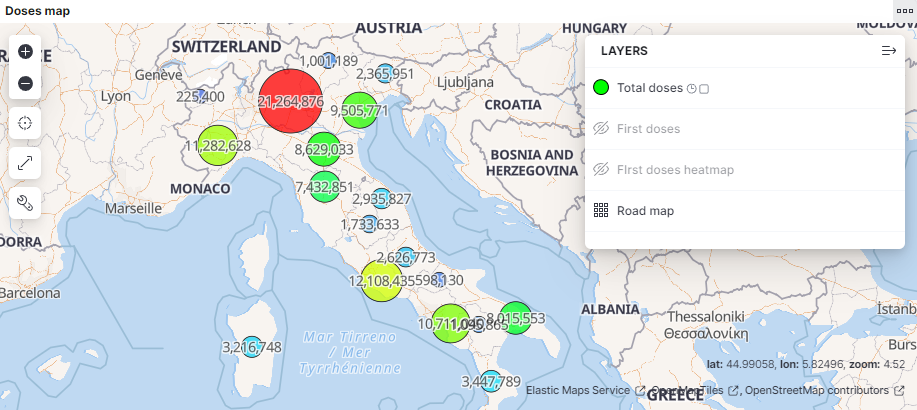
\includegraphics[width=1\textwidth, frame]{Doses_map.PNG}
    \caption{Map of vaccine's doses delivered and administered from the beginning of the campaign}
\end{center}
\end{figure}

\newpage

\section{Queries \& Commands}\label{cmd-que}

\subsection{Queries}

The following subsection presents some useful queries and their possible textual result, with the aim of showing database's utility

\subsubsection{Daily number of overall, first, second and booster vaccine doses}\label{ssec:q1}

Note that this query has a dedicated dashboard's panel, as explained in subsection \ref{ssec:dash3}

\begin{figure}[H]
\begin{center}
\begin{minipage}[b]{0.4\textwidth}
    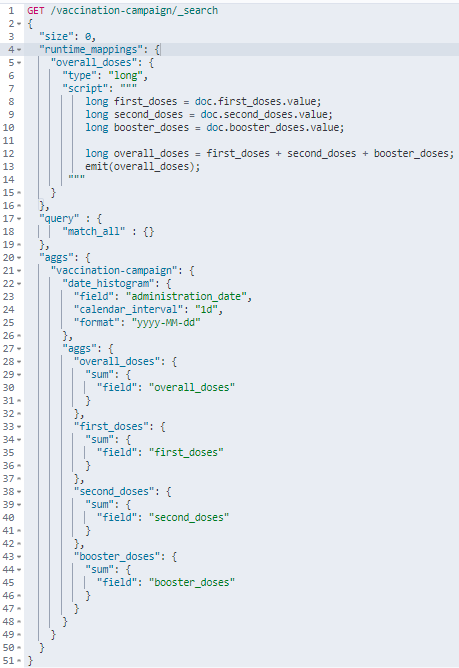
\includegraphics[width=\textwidth, frame]{Query_1.PNG}
    \subcaption{}
  \end{minipage}
  \hfill
  \begin{minipage}[b]{0.4\textwidth}
    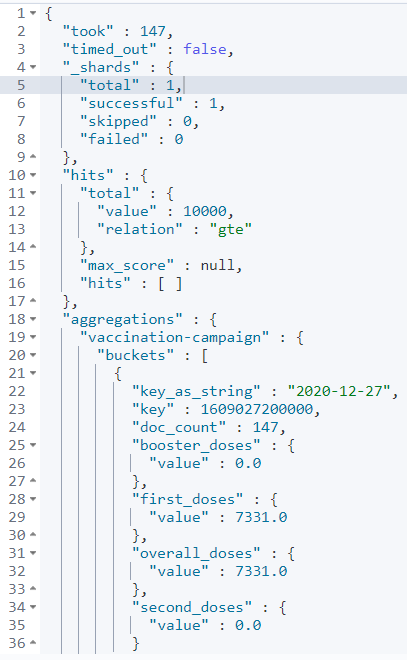
\includegraphics[width=\textwidth, frame]{Answer_Query_1.PNG}
     \subcaption{}
  \end{minipage}
  \caption{(a) shows the query, while (b) shows a portion of the result}
\end{center}
\end{figure}

With little modification to the above query, we can obtain interesting results. If we want to group to filter by region-name, we can simply add: 
\begin{figure}[H]
    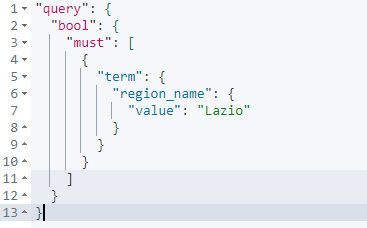
\includegraphics[width=0.4\textwidth, frame]{Query_1.1.png}
\end{figure}
If instead we would like to group by region-name, we can add outside the "aggs" of "vaccination-campaign" this other aggregation:
\begin{figure}[H]
    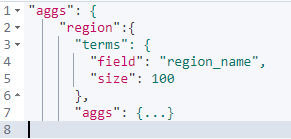
\includegraphics[width=0.4\textwidth, frame]{Query_1,2.png}
\end{figure}

Further examples (with different starting queries) showing this features are provided in the next queries.

\subsubsection{COVID-19 Overall vaccine doses administered}\label{ssec:q2}


\begin{figure}[H]
\begin{center}
\begin{minipage}[b]{0.4\textwidth}
    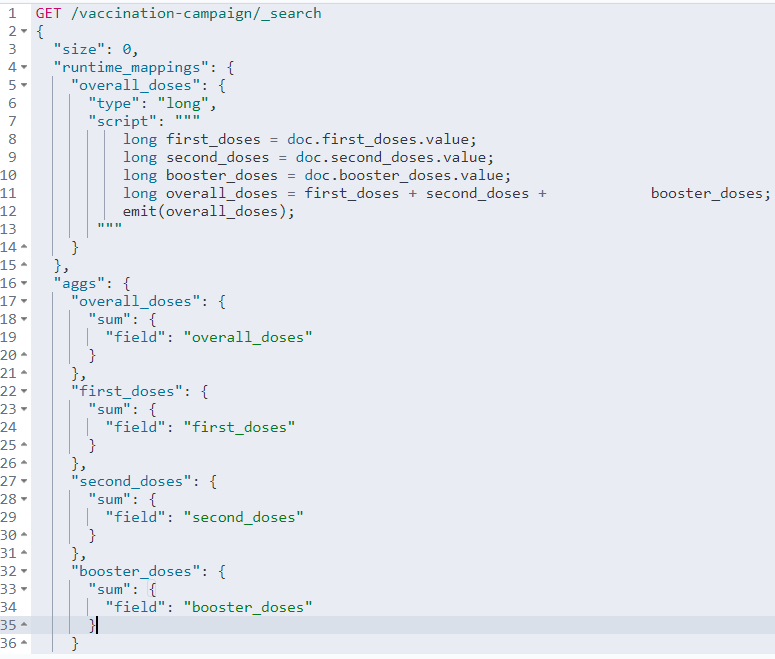
\includegraphics[width=\textwidth, frame]{Query_2.PNG}
    \subcaption{}
  \end{minipage}
  \hfill
  \begin{minipage}[b]{0.4\textwidth}
    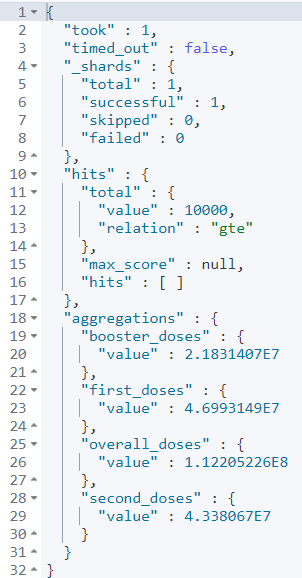
\includegraphics[width=\textwidth, frame]{Answer_Query_2.PNG}
     \subcaption{}
  \end{minipage}
  \caption{(a) shows the query, while (b) shows a portion of the result}
\end{center}
\end{figure}

\newpage

\subsubsection{Gender distribution of weekly vaccine doses administered}\label{ssec:q3}


Note that this query has a dedicated dashboard's panel, as explained in section \ref{ssec:dash1}.

\begin{figure}[H]
\begin{center}
\begin{minipage}[b]{0.4\textwidth}
    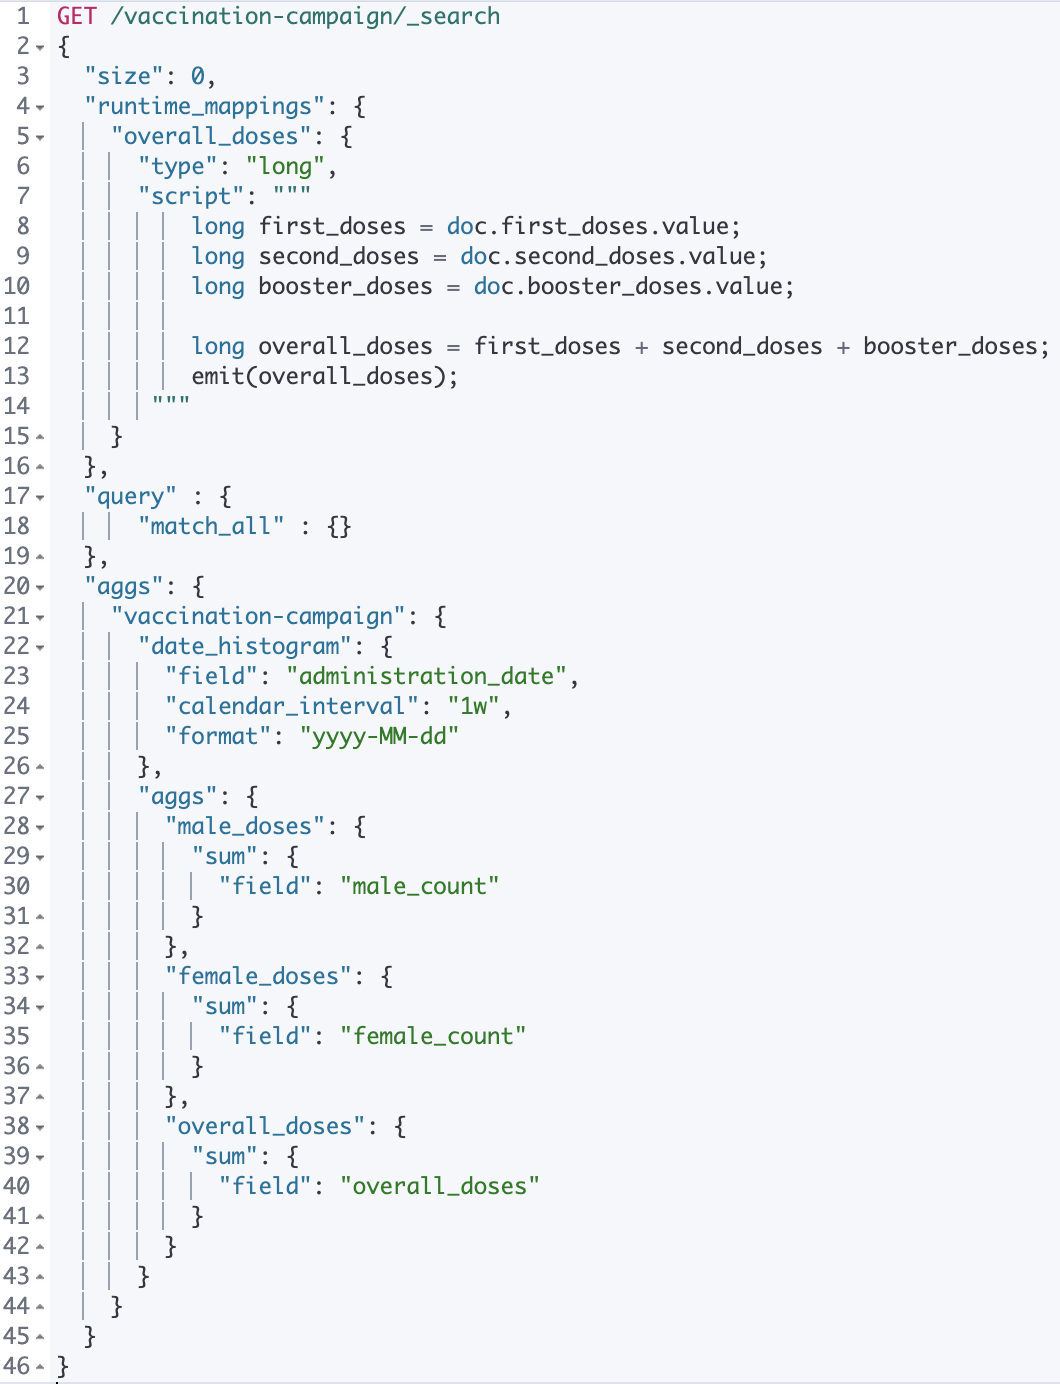
\includegraphics[width=\textwidth, frame]{Query_4BIS.PNG}
    \subcaption{}
  \end{minipage}
  \hfill
  \begin{minipage}[b]{0.4\textwidth}
    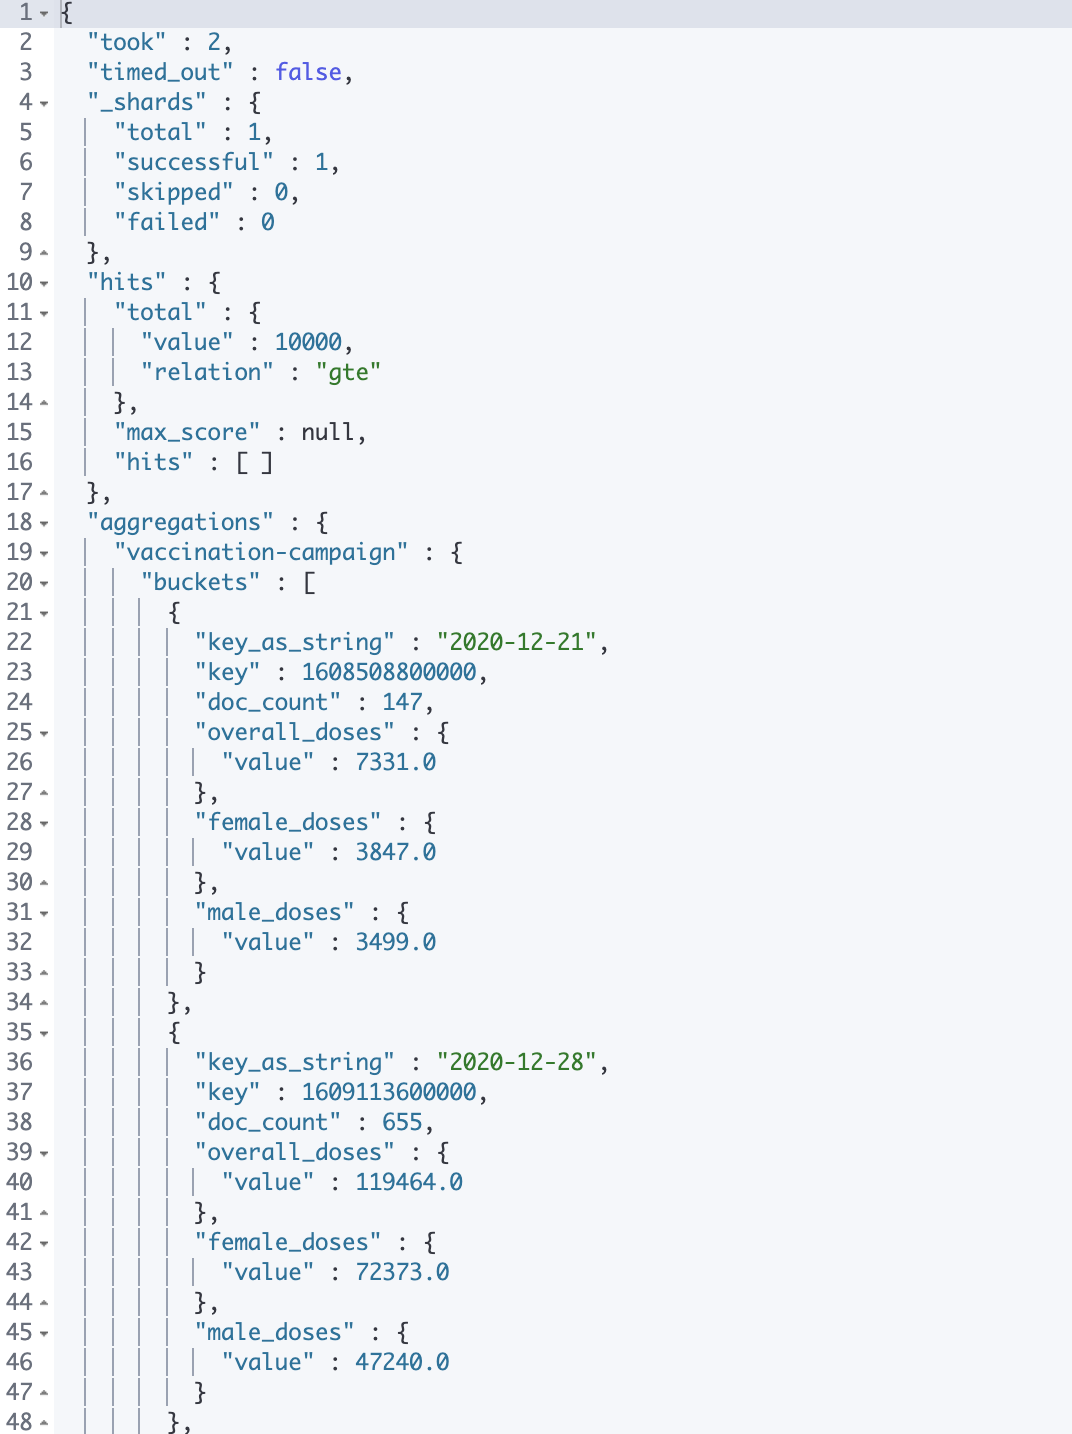
\includegraphics[width=\textwidth, frame]{Answer_Query_4BIS.PNG}
     \subcaption{}
  \end{minipage}
  \caption{(a) shows the query, while (b) shows a portion of the result}
\end{center}
\end{figure}

\newpage

\subsubsection{Suppliers distribution percentage of all administered vaccines}\label{ssec:q4}


Note that this query has a dedicated dashboard's panel, as explained in section \ref{ssec:dash5}.

\begin{figure}[H]
\begin{center}
\begin{minipage}[b]{0.4\textwidth}
    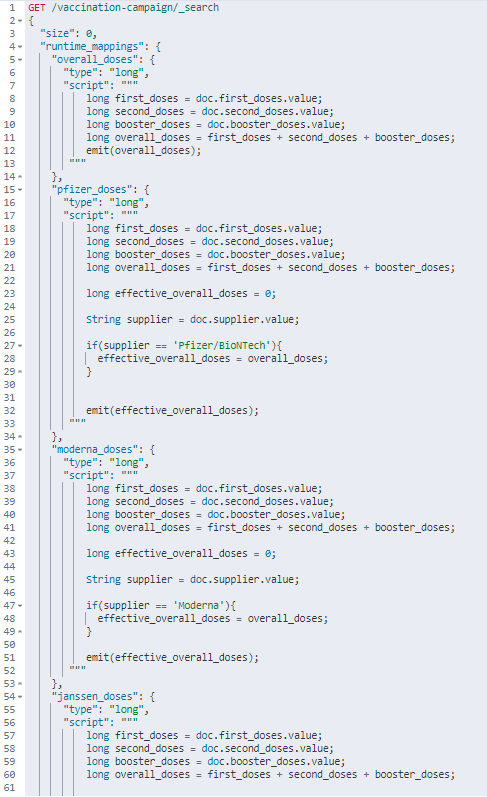
\includegraphics[width=0.8\textwidth, frame]{Query_2BIS_1.PNG}
    \subcaption{}
  \end{minipage}
  \hfill  
\begin{minipage}[b]{0.4\textwidth}
    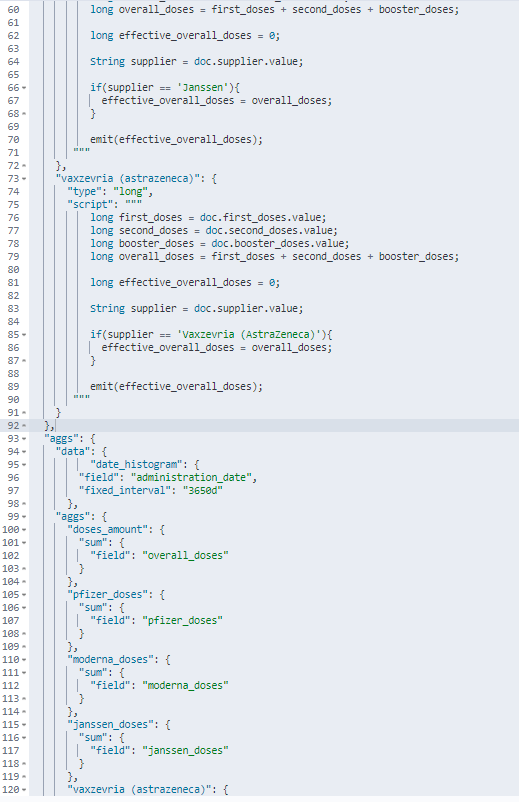
\includegraphics[width=0.8\textwidth, frame]{Query_2BIS_2.PNG}
     \subcaption{}
\end{minipage}

\begin{minipage}[b]{0.4\textwidth}
    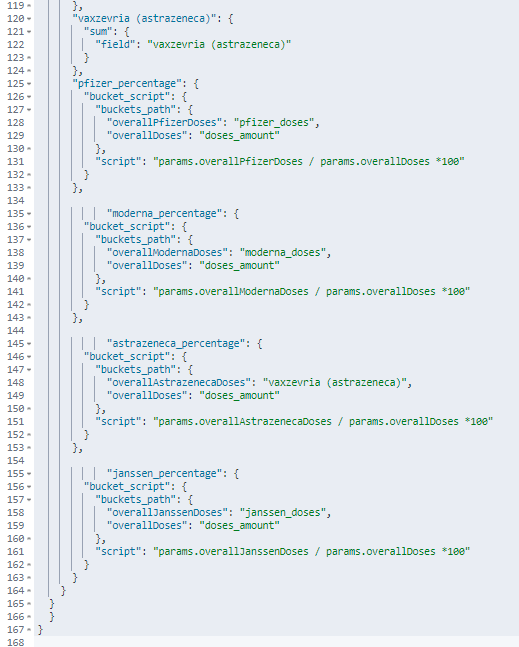
\includegraphics[width=0.8\textwidth, frame]{Query_2BIS_3.PNG}
     \subcaption{}
  \end{minipage}
    \hfill 
\begin{minipage}[b]{0.4\textwidth}
    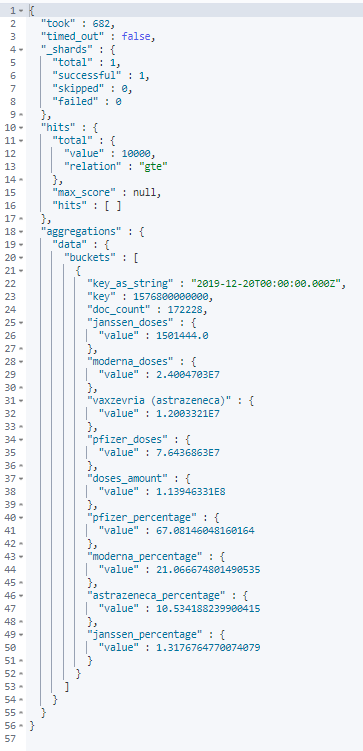
\includegraphics[width=0.8\textwidth, frame]{Answer_Query_2BIS.png}
     \subcaption{}
  \end{minipage}
  \caption{(a), (b), (c) show the query, while (d) shows a portion of the result}
\end{center}
\end{figure}

\subsubsection{Number of people that have received at least one dose by age range.}\label{ssec:q5}


\begin{figure}[H]
\begin{center}
\begin{minipage}[b]{0.4\textwidth}
    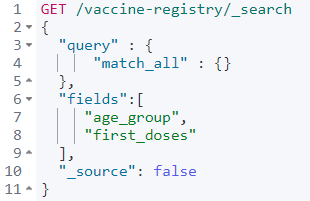
\includegraphics[width=\textwidth, frame]{Query_3.PNG}
    \subcaption{}
  \end{minipage}
  \hfill
  \begin{minipage}[b]{0.4\textwidth}
    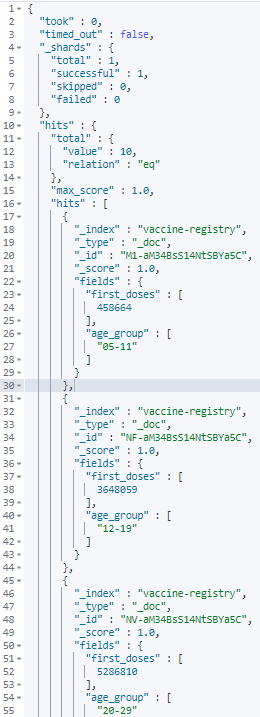
\includegraphics[width=\textwidth, frame]{Answer_Query_3.PNG}
     \subcaption{}
  \end{minipage}
  \caption{(a) shows the query, while (b) shows a portion of the result}
\end{center}
\end{figure}

\newpage

\subsubsection{Get vaccination status of all age groups}\label{ssec:q6}


Note that this query has a dedicated dashboard's panel, as explained in section \ref{ssec:dash6}

\begin{figure}[H]
\begin{center}
\begin{minipage}[b]{0.4\textwidth}
    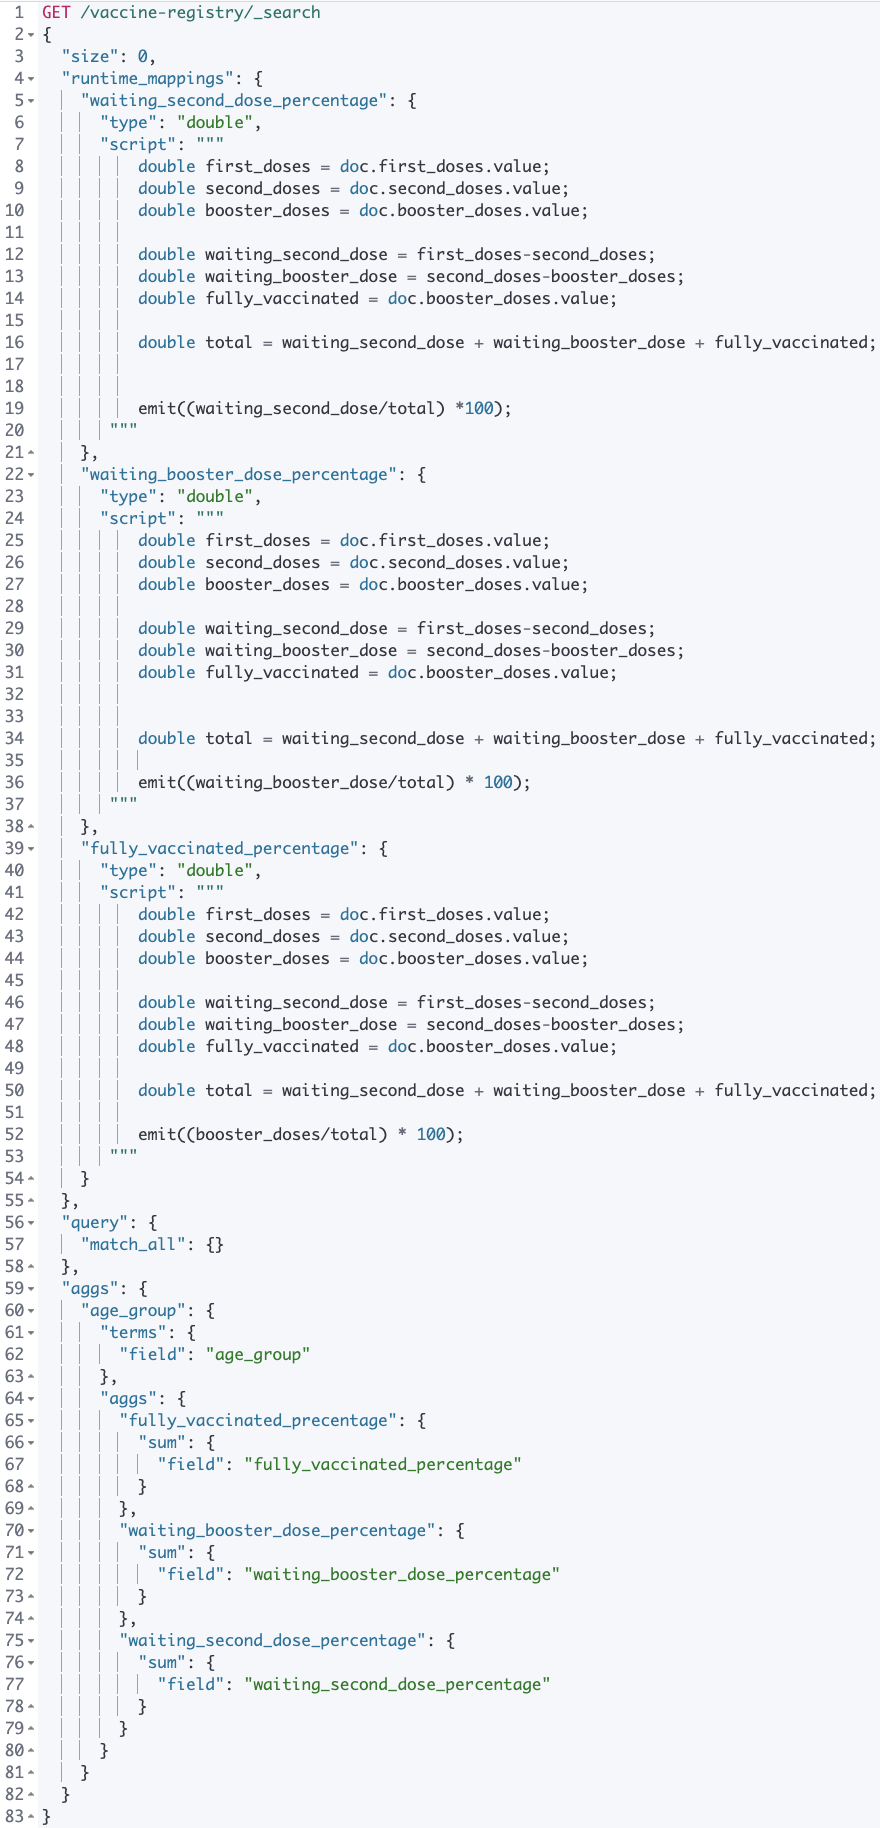
\includegraphics[width=0.9\textwidth, frame]{Query_9BIS.png}
    \subcaption{}
  \end{minipage}
  \hfill
  \begin{minipage}[b]{0.4\textwidth}
    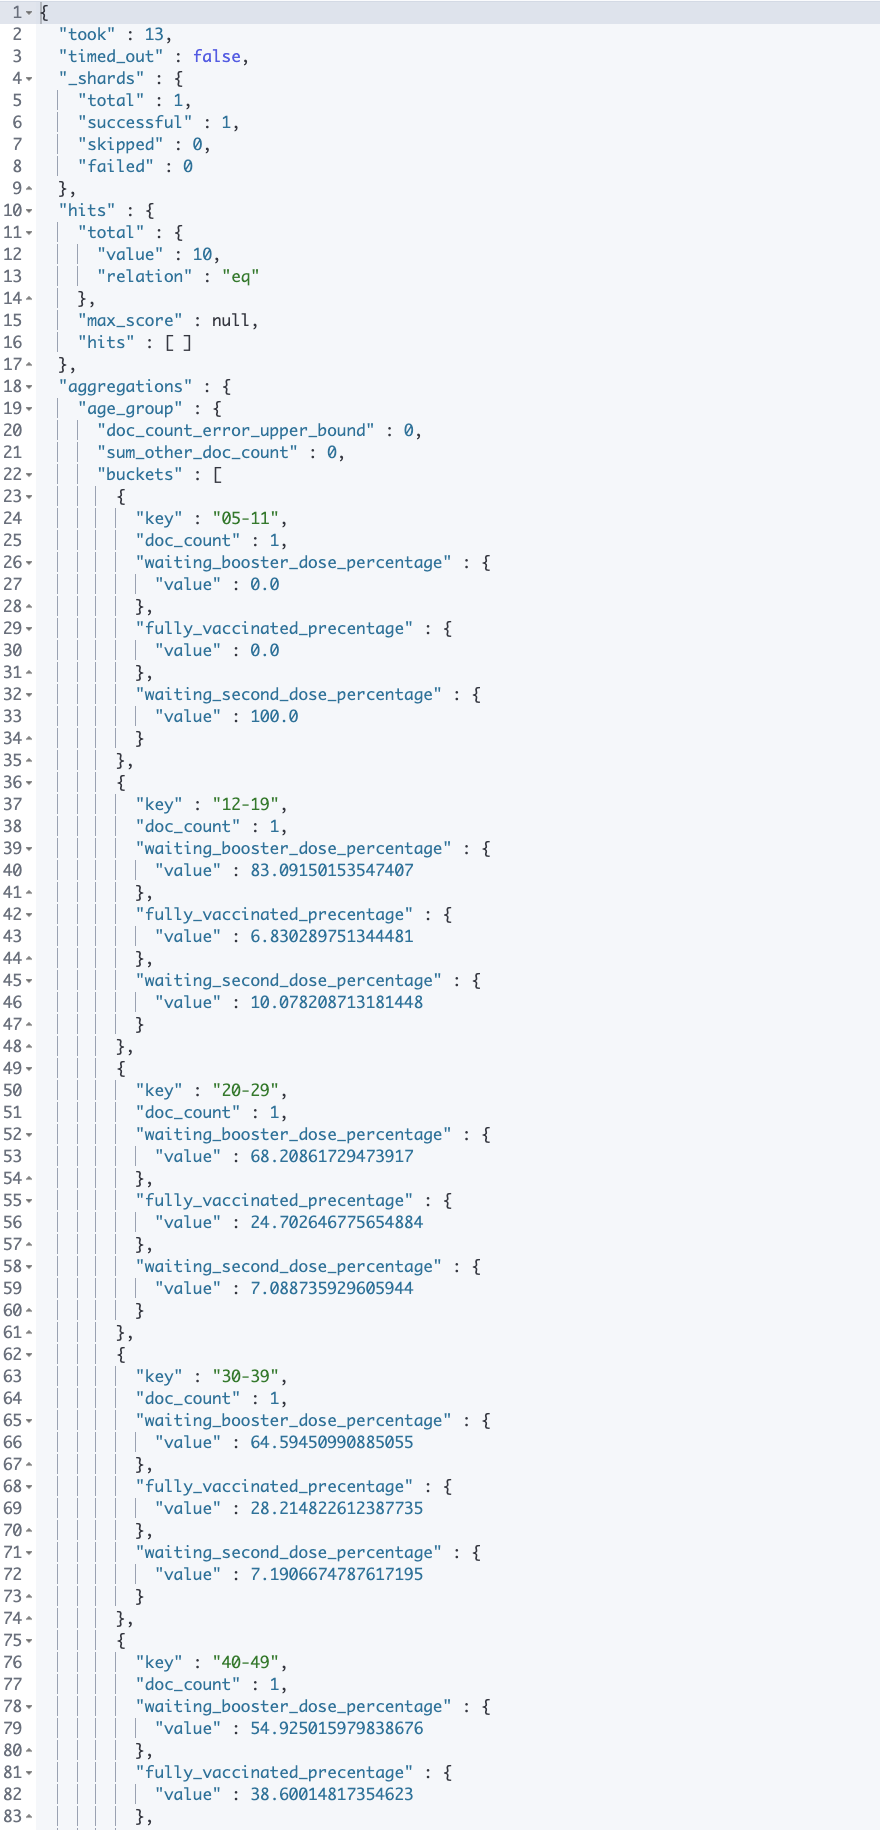
\includegraphics[width=0.9\textwidth, frame]{Answer_Query_9BIS.png}
     \subcaption{}
  \end{minipage}
  \caption{(a) shows the query, while (b) shows a portion of the result}
\end{center}
\end{figure}



\subsubsection{Get the total number of not vaccinated people}\label{ssec:q7}


Note that this query has a dedicated dashboard's panel, as explained in section \ref{ssec:dash2}

\begin{figure}[H]
\begin{center}
\begin{minipage}[b]{0.4\textwidth}
    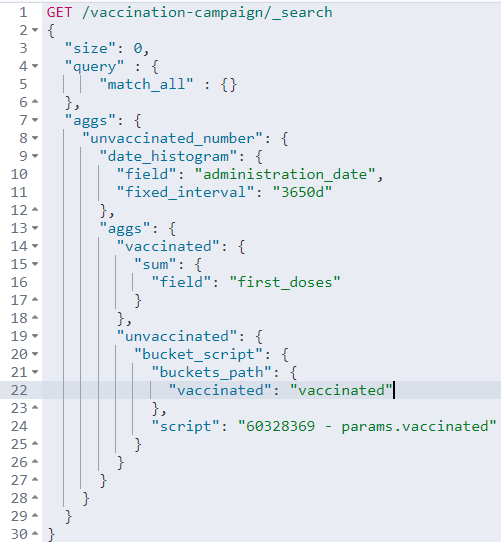
\includegraphics[width=0.9\textwidth, frame]{Query_7.PNG}
    \subcaption{}
  \end{minipage}
  \hfill
  \begin{minipage}[b]{0.4\textwidth}
    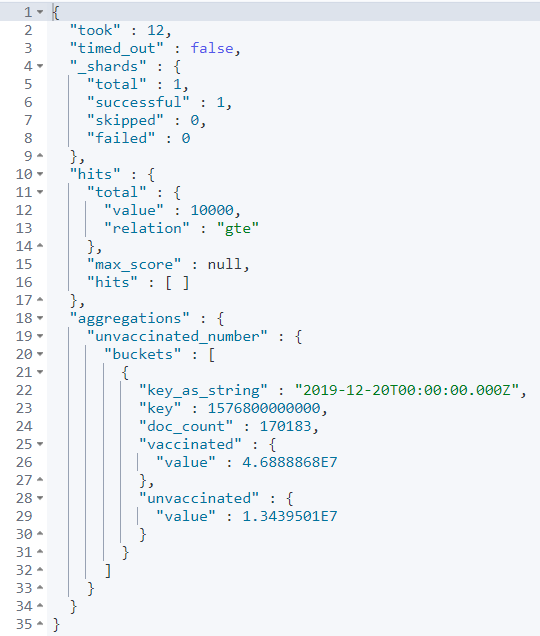
\includegraphics[width=0.9\textwidth, frame]{Answer_Query_7.PNG}
     \subcaption{}
  \end{minipage}
  \caption{(a) shows the query, while (b) shows a portion of the result}
\end{center}
\end{figure}

\subsubsection{Get the number of vaccinated people that still have to take the booster dose}\label{ssec:q8}


\begin{figure}[H]
\begin{center}
\begin{minipage}[b]{0.4\textwidth}
    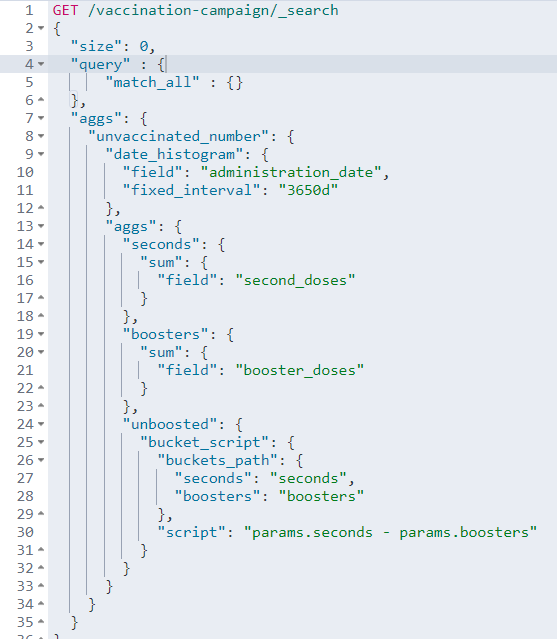
\includegraphics[width=\textwidth, frame]{Query_8.PNG}
    \subcaption{}
  \end{minipage}
  \hfill
  \begin{minipage}[b]{0.4\textwidth}
    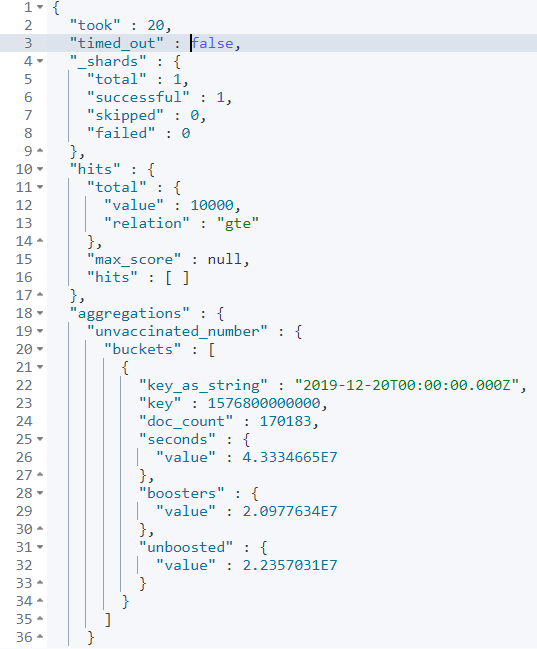
\includegraphics[width=\textwidth, frame]{Answer_Query_8.PNG}
     \subcaption{}
  \end{minipage}
  \caption{(a) shows the query, while (b) shows a portion of the result}
\end{center}
\end{figure}

\subsubsection{Get the number of people that have been tested positive in the previous 3/6 months and so needed only one dose of vaccine, by age-group}\label{ssec:q9}


\begin{figure}[H]
\begin{center}
\begin{minipage}[b]{0.4\textwidth}
    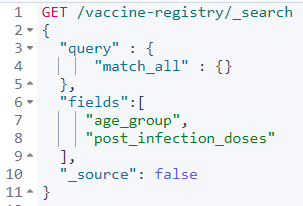
\includegraphics[width=\textwidth, frame]{Query_9.PNG}
    \subcaption{}
  \end{minipage}
  \hfill
  \begin{minipage}[b]{0.4\textwidth}
    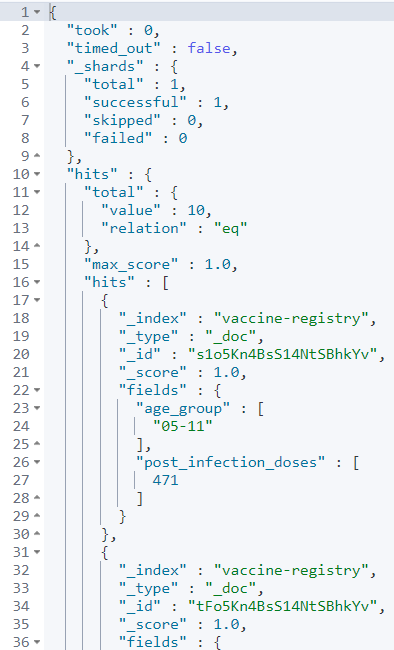
\includegraphics[width=\textwidth, frame]{Answer_Query_9.PNG}
     \subcaption{}
  \end{minipage}
  \caption{(a) shows the query, while (b) shows a portion of the result}
\end{center}
\end{figure}

\subsubsection{Get the male percentage of administered vaccines by date}\label{ssec:q10}


\begin{figure}[H]
\begin{center}
\begin{minipage}[b]{0.4\textwidth}
    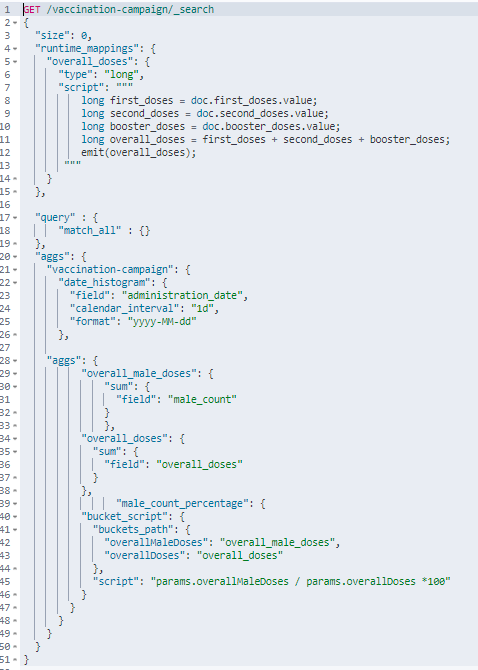
\includegraphics[width=\textwidth, frame]{Query_4.PNG}
    \subcaption{}
  \end{minipage}
  \hfill
  \begin{minipage}[b]{0.4\textwidth}
    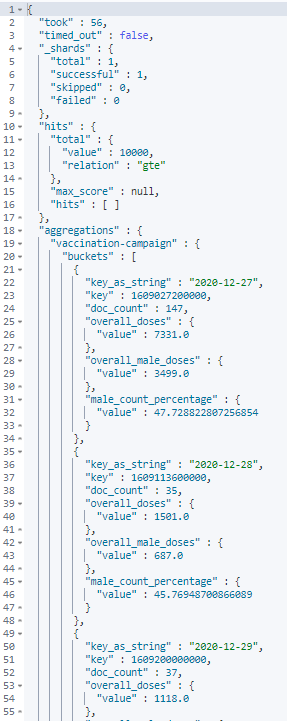
\includegraphics[width=\textwidth, frame]{Answer_Query_4.PNG}
     \subcaption{}
  \end{minipage}
  \caption{(a) shows the query, while (b) shows a portion of the result}
\end{center}
\end{figure}

\newpage

\subsubsection{Get total doses delivered by each supplier}\label{ssec:q11}


\begin{figure}[H]
\begin{center}
\begin{minipage}[b]{0.4\textwidth}
    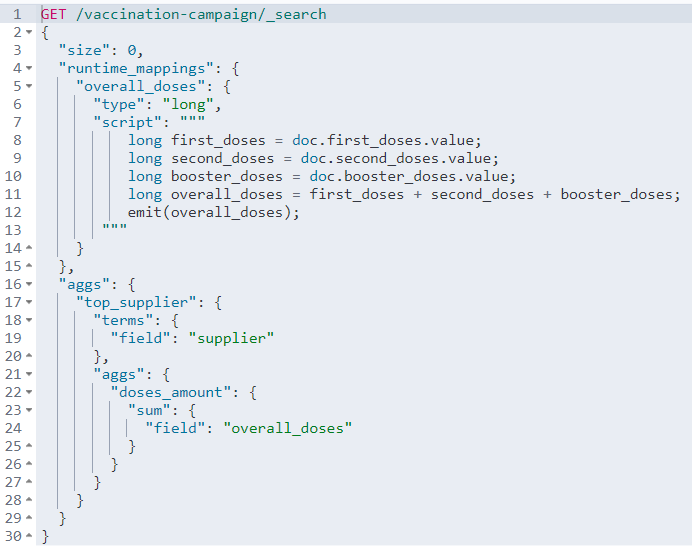
\includegraphics[width=\textwidth, frame]{Query_5.PNG}
    \subcaption{}
  \end{minipage}
  \hfill
  \begin{minipage}[b]{0.4\textwidth}
    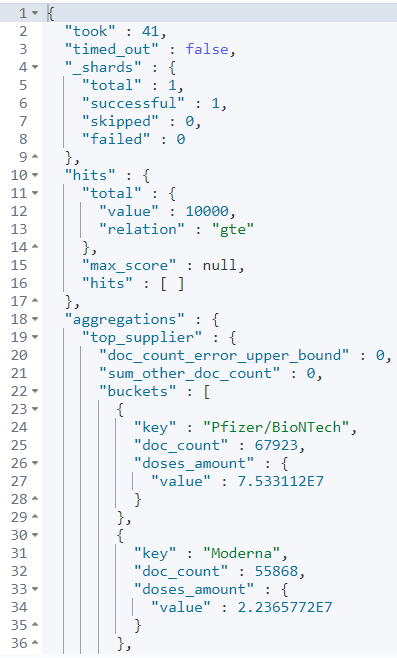
\includegraphics[width=\textwidth, frame]{Answer_Query_5.PNG}
     \subcaption{}
  \end{minipage}
  \caption{(a) shows the query, while (b) shows a portion of the result}
\end{center}
\end{figure}

\newpage

\subsubsection{Get the increase in percentage of vaccines done related to the previous day}\label{ssec:q12}


\begin{figure}[H]
\begin{center}
\begin{minipage}[b]{0.4\textwidth}
    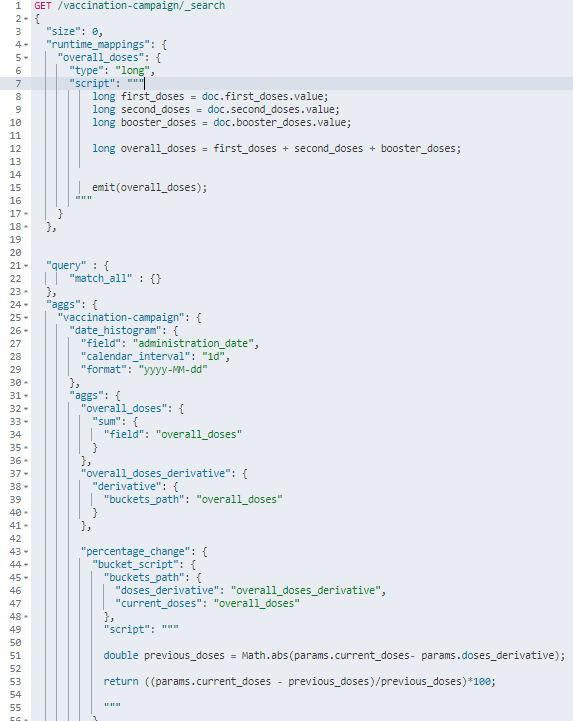
\includegraphics[width=\textwidth, frame]{Query_6.PNG}
    \subcaption{}
  \end{minipage}
  \hfill
  \begin{minipage}[b]{0.4\textwidth}
    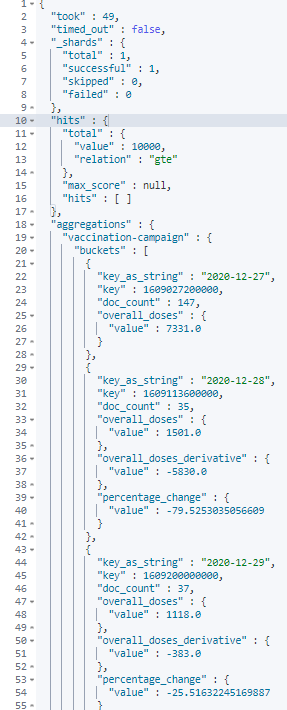
\includegraphics[width=\textwidth, frame]{Answer_Query_6.PNG}
     \subcaption{}
  \end{minipage}
  \caption{(a) shows the query, while (b) shows a portion of the result}
\end{center}
\end{figure}

\newpage

\subsubsection{Get the overall number of doses delivered}\label{ssec:q13}

Note that this query has a dedicated dashboard's panel, as explained in section \ref{ssec:dash4}

\begin{figure}[H]
\begin{center}
\begin{minipage}[b]{0.4\textwidth}
    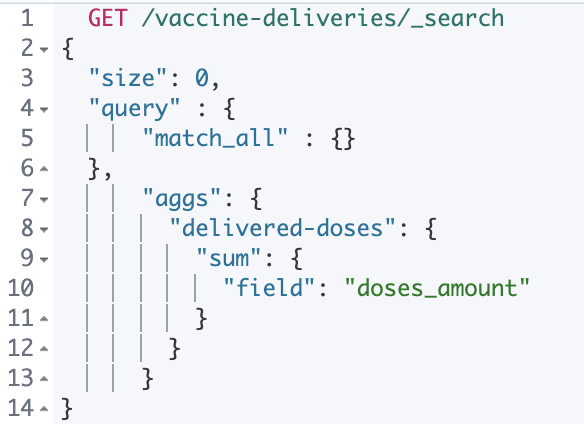
\includegraphics[width=0.8\textwidth, frame]{Query_13.PNG}
    \subcaption{}
  \end{minipage}
  \hfill
  \begin{minipage}[b]{0.4\textwidth}
    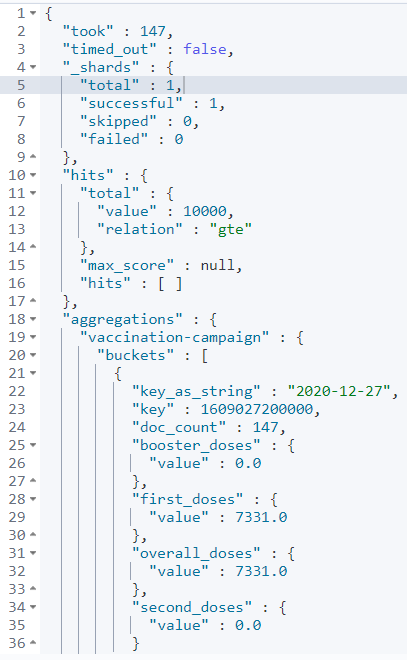
\includegraphics[width=0.8\textwidth, frame]{Answer_Query_1.PNG}
     \subcaption{}
  \end{minipage}
  \caption{(a) shows the query, while (b) shows a portion of the result}
\end{center}
\end{figure}


\subsubsection{Get overall weekly vaccine deliveries amount}\label{ssec:q14}


\begin{figure}[H]
\begin{center}
\begin{minipage}[b]{0.4\textwidth}
    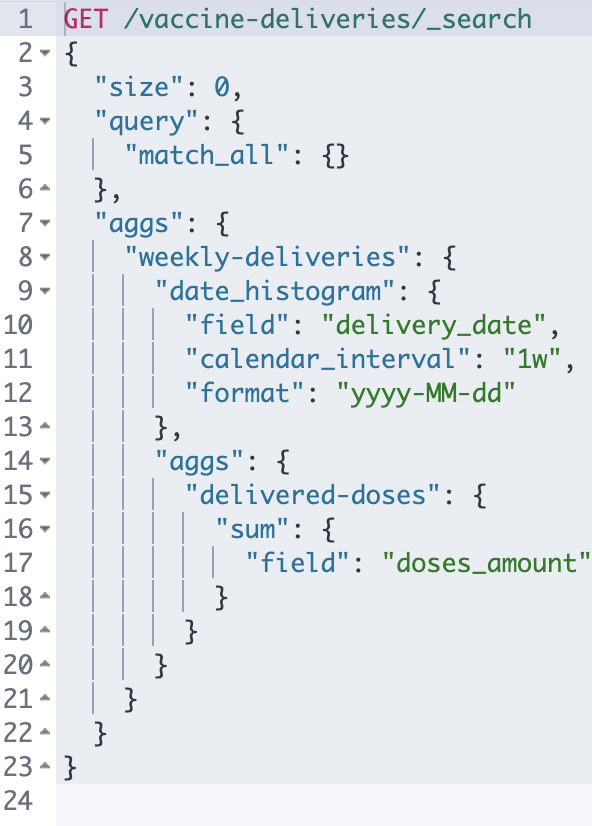
\includegraphics[width=0.8\textwidth, frame]{Query_10.PNG}
    \subcaption{}
  \end{minipage}
  \hfill
  \begin{minipage}[b]{0.4\textwidth}
    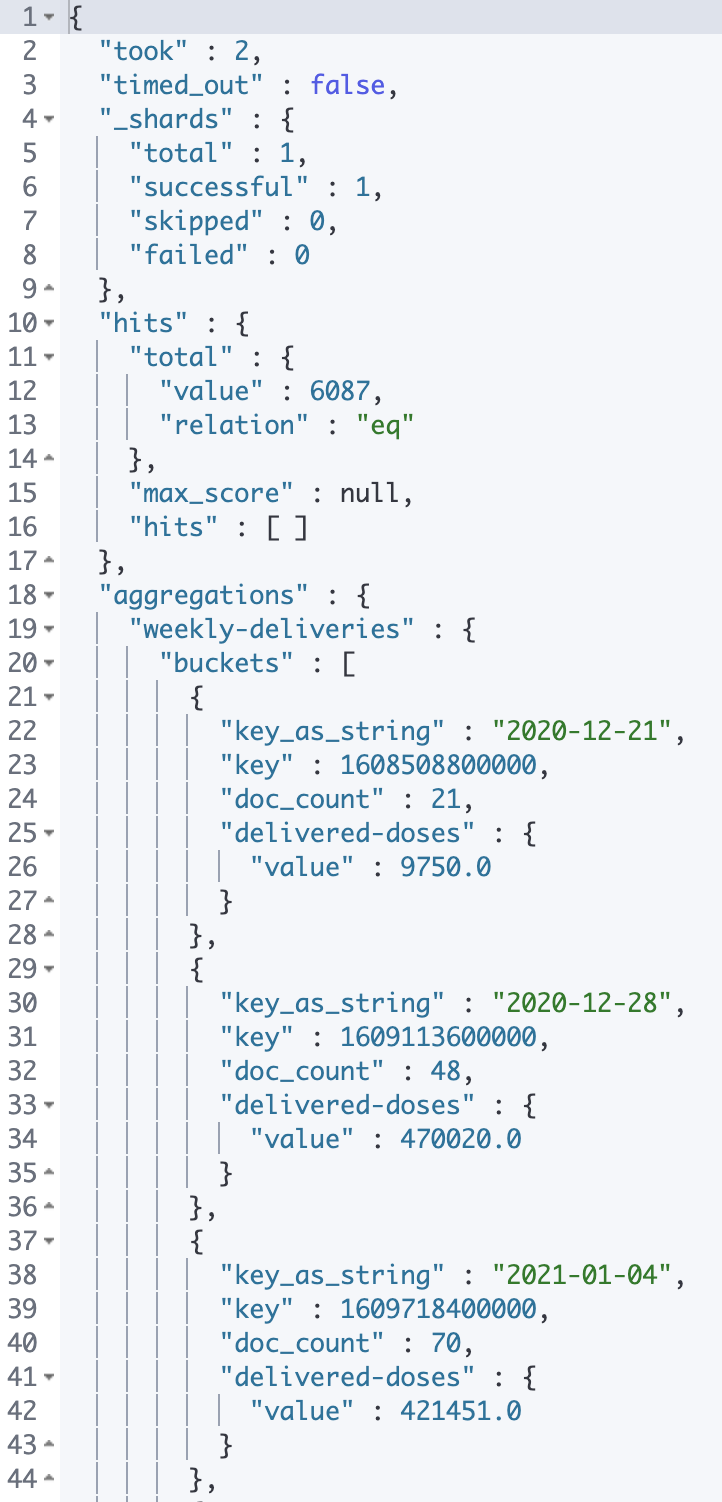
\includegraphics[width=0.8\textwidth, frame]{Answer_Query_10.PNG}
     \subcaption{}
  \end{minipage}
  \caption{(a) shows the query, while (b) shows a portion of the result}
\end{center}
\end{figure}

\subsubsection{Get vaccine deliveries amount by region name}\label{ssec:q15}

\begin{figure}[H]
\begin{center}
\begin{minipage}[b]{0.4\textwidth}
    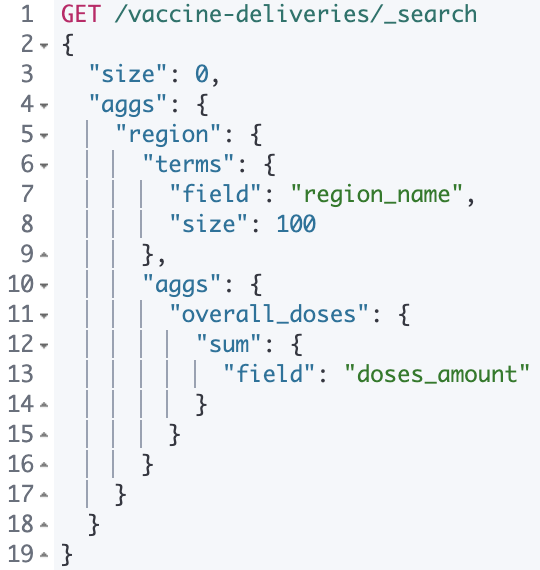
\includegraphics[width=\textwidth, frame]{Query_11.PNG}
    \subcaption{}
  \end{minipage}
  \hfill
  \begin{minipage}[b]{0.4\textwidth}
    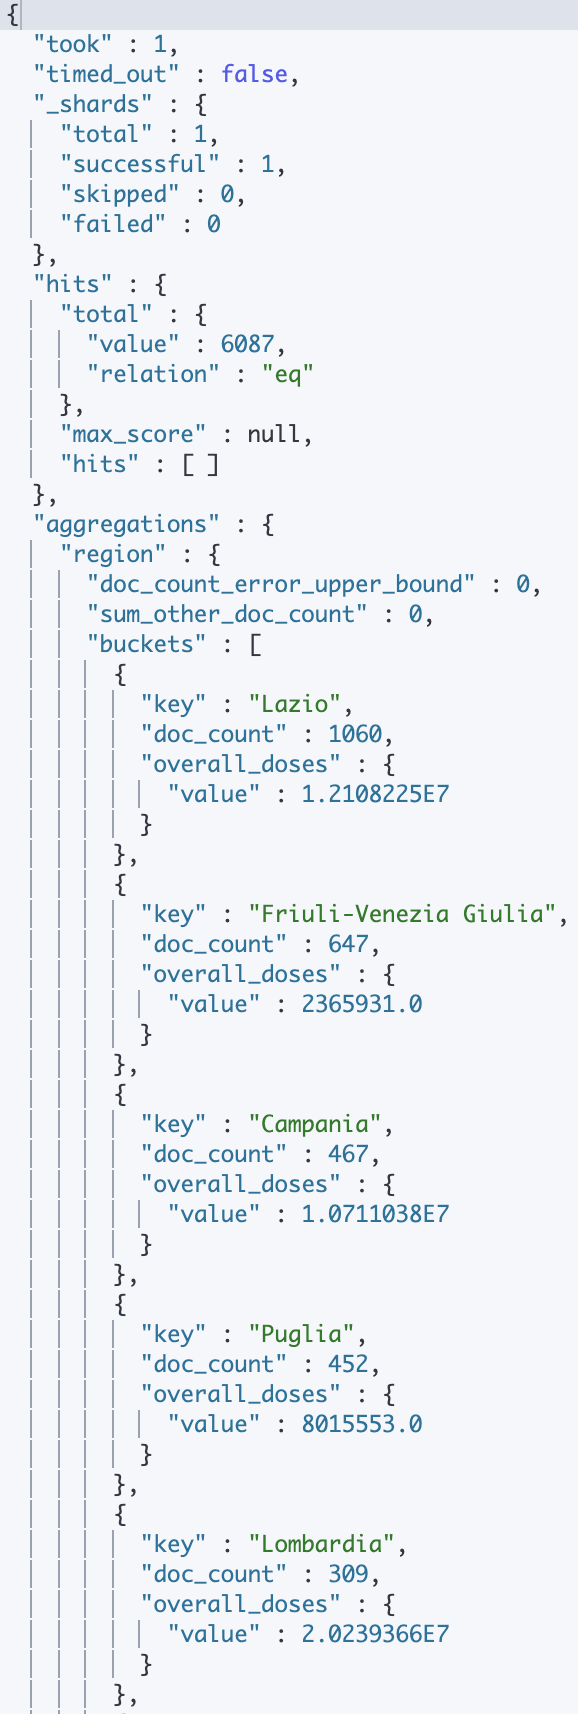
\includegraphics[width=\textwidth, frame]{Answer_Query_11.PNG}
     \subcaption{}
  \end{minipage}
  \caption{(a) shows the query, while (b) shows a portion of the result}
\end{center}
\end{figure}

\subsubsection{Get weekly vaccine deliveries amount by manufacturer}\label{ssec:q16}


\begin{figure}[H]
\begin{center}
\begin{minipage}[b]{0.4\textwidth}
    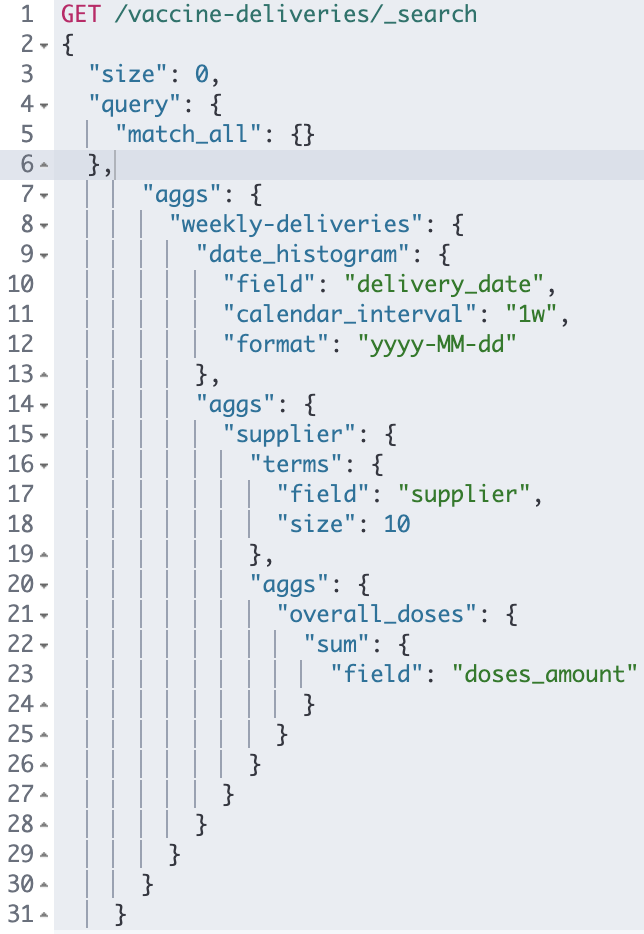
\includegraphics[width=\textwidth, frame]{Query_12.PNG}
    \subcaption{}
  \end{minipage}
  \hfill
  \begin{minipage}[b]{0.4\textwidth}
    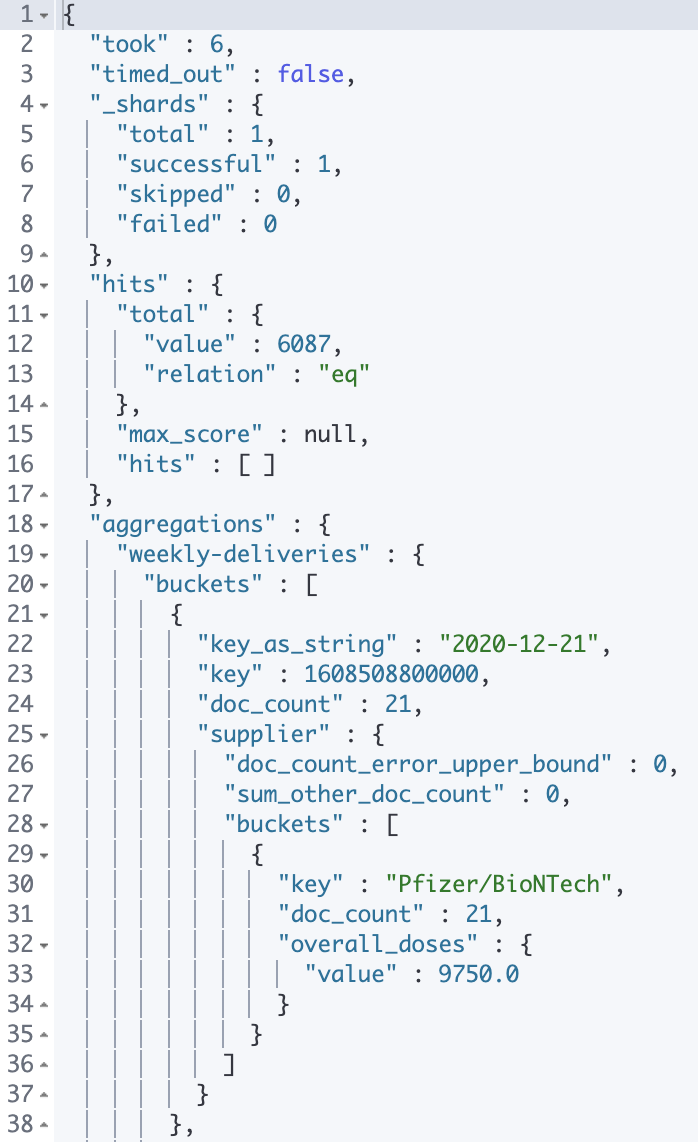
\includegraphics[width=\textwidth, frame]{Answer_Query_12.PNG}
     \subcaption{}
  \end{minipage}
  \caption{(a) shows the query, while (b) shows a portion of the result}
\end{center}
\end{figure}

\subsection{Commands}

\subsubsection{Delete all documents related to 2020 from vaccine campaign index}

\begin{figure}[H]
\begin{center}
\begin{minipage}[b]{0.4\textwidth}
    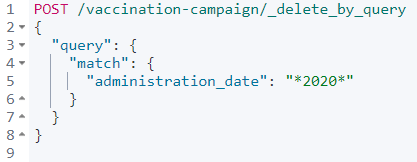
\includegraphics[width=\textwidth, frame]{Command_1.png}
  \end{minipage}
  \hfill
  \caption{shows the deletion command}
\end{center}
\end{figure}

\subsubsection{Insert a new document into vaccine registry index}

\begin{figure}[H]
\begin{center}
\begin{minipage}[b]{0.4\textwidth}
    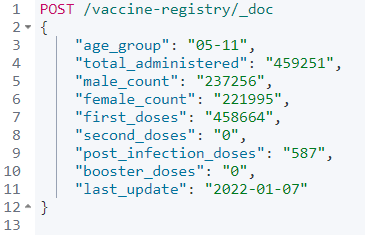
\includegraphics[width=\textwidth, frame]{Command_2.png}
  \end{minipage}
  \hfill
  \caption{shows the insertion command}
\end{center}
\end{figure}

\appendix
\section{Delivery content}
Apart from this report, the delivery folder also contains the following files :
\begin{itemize}
    \item \textbf{Python scripts} to create CSVs and indexes. The Python project is mainly composed by 5 files
    \begin{itemize}
        \item \textbf{utils.py}: it contains various utility functions manipulate CSV files and to retrive files from Github repository.
        \item \textbf{main.py}: it contains functions to handle the daily routine.
        \item \textbf{constants.py}: it contains all the various constants, such as api keys, enums and files' paths, used among different functions.
        \item \textbf{elasticutils.py}: it contains utility functions related to Elasticsearch, to create \& delete indexes, create data mappings and upload data.
        \item \textbf{csvmanipulation.py}:  it contains various utility functions manipulate CSV files.
        \item \textbf{setup.ini}: configuration file holding information about files' paths and Elasticsearch/GMaps connection API keys. 
        
    \end{itemize}
    \item \textbf{Folders} containing the various versions of CSVs files, to keep track of the subsequent modifications (these are located inside the Python project folder, inside the \textbf{datasets} folder) (note that in case of files deletion, these will be automatically recreated through \textbf{main.py} executable file)
    \item \textbf{Elasticsearch indexes}.
    \item \textbf{Text file} with queries\&commands.
    \item \textbf{Kibana Complete dashboard \& Single graphs} files.
\end{itemize}

%===========================================================
%===========================================================

\begin{thebibliography}{00}

\bibitem{b1}Google Maps API - \url{https://developers.google.com/maps/documentation/geocoding/overview}
\bibitem{b2}ELK stack - \url{https://www.elastic.co/what-is/elk-stack}
\bibitem{b3}Elasticsearch - \url{https://www.postdicom.com/it}
\bibitem{b4}Kibana - \url{https://www.elastic.co/kibana/}
\bibitem{b5}Python \url{https://www.python.org}
\bibtem{b6}Github File Watched \url{https://app.github-file-watcher.com}

\end{thebibliography}


\end{document}